%%%%%%%%%%%%%%%%%%%%%%% file template.tex %%%%%%%%%%%%%%%%%%%%%%%%%
%
% This is a template file for the LaTeX package SVJour2 for the
% Springer journal "Biological Cybernetics"
%
%                                    Springer Heidelberg 2004/11/22
%
% Copy it to a new file with a new name and use it as the basis
% for your article
%
%%%%%%%%%%%%%%%%%%%%%%%%%%%%%%%%%%%%%%%%%%%%%%%%%%%%%%%%%%%%%%%%%%%
%
% First comes an example EPS file -- just ignore it and
% proceed on the \documentclass line
% your LaTeX will extract the file if required
\begin{filecontents*}{example.eps}
%!PS-Adobe-3.0 EPSF-3.0
%%BoundingBox: 19 19 221 221
%%CreationDate: Mon Sep 29 1997
%%Creator: programmed by hand (JK)
%%EndComments
gsave
newpath
  20 20 moveto
  20 220 lineto
  220 220 lineto
  220 20 lineto
closepath
2 setlinewidth
gsave
  .4 setgray fill
grestore
stroke
grestore
\end{filecontents*}
%
\documentclass[twocolumn,fleqn]{svjour3}
% Biological Cybernetics uses author year
% references, hence the natbib package is activated - use
% \citet{...} and \citep{...} with it to cite references.
%
\smartqed  % flush right qed marks, e.g. at end of proof
%
\usepackage[numbers]{natbib}
\usepackage{amssymb}
\usepackage{amsmath}
\usepackage{textcomp}
\usepackage[T1]{fontenc}
\usepackage[utf8]{inputenc}
\usepackage[spanish]{babel}
\usepackage{csquotes}
\usepackage{enumerate}
\usepackage{enumitem}
\usepackage{caption}
\captionsetup{compatibility=false}
\usepackage{subcaption}
\usepackage{listings}
% para la lista de simbolos
\usepackage{array} %for vertical thick lines in tables
\usepackage{multirow} %multirow tables
\usepackage{nicefrac} %for fractions like 1/4
\usepackage[dvipsnames]{xcolor}
\usepackage{pgfplots}
\pgfplotsset{compat=default}
\usepackage{pgfplotstable}
\usepgfplotslibrary{statistics}
\usetikzlibrary{spy}
\usepackage{longtable}
\usepackage{array}
\usepackage{pdflscape}
\usepackage{booktabs}



%
% \usepackage{mathptmx}      % use Times fonts if available on your TeX system
%
% insert here the call for the packages your document requires
%\usepackage{latexsym}
% etc.
%
% please place your own definitions here and don't use \def but
% \newcommand{}{}
%
\journalname{}

\DeclareUnicodeCharacter{2217}{*}

%
\begin{document}

\title{Ordenamiento de colores RGB basado en m\'etricas asociadas a la imagen  %\thanks{Grants or other notes
%about the article that should go on the front page should be
%placed here. General acknowledgments should be placed at the end of the article.}
}
%\subtitle{Do you have a subtitle?\\ If so, write it here}

%\titlerunning{Short form of title}        % if too long for running head

\author{Jos\'e Luis V\'azquez Noguera \and
        Christian E. Schaerer \and
				Jacques Facon	\and %etc.
        Horacio Legal Ayala
				}

%\authorrunning{Short form of author list} % if too long for running head

\institute{Jos\'e Luis V\'azquez Noguera  $\cdot$ Christian E. Schaerer \at  
              Polytechnic Faculty, National University of Asuncion - San Lorenzo, Paraguay \\
              %Tel.: +123-45-678910\\
              %Fax: +123-45-678910\\
              \email{\{jlvazquez,hlegal,cschaer\}@pol.una.py}           %  \\
%             \emph{Present address:} of F. Author  %  if needed
           \and
           Jacques Facon \at
              PPGIa - PUCPR-Pontif´ıcia Universidade Catolica do Paran ´ a - Curitiba - Pr, Brazil \\
              %Tel.: +123-45-678910\\
              %Fax: +123-45-678910\\
              \email{facon@ppgia.pucpr.br}  
}

\date{Received: date / Revised: date}
% The correct dates will be entered by the editor
\maketitle

\begin{abstract}
El orden lexicogr\'afico y sus variantes son los m\'as utilizados en la literatura para el ordenamiento de colores.  Un problema usual de este tipo de ordenamiento es el establececimiento a priori del componente de color m\'as importante y el resultado de las comparaciones lexicogr\'aficas casi siempre se deciden en los primeros componentes.  La norma o la distancia a un color de referencia es tambi\'en bastante utilizado como estrategia de ordenamiento, pero en las im\'agenes a color RGB dos colores visuales distintos pueden tener la misma norma, o distancia a un color de referencia. Debido a que no existe un orden natural entre los colores RGB ser\'ia de utilidad encontrar una estrategia de ordenamiento que sea dependiente de la imagen y de la aplicaci\'on. En este art\'iculo se propone un  ordenamiento en el cu\'al se asigna una ponderaci\'on a cada componente de color de acuerdo a m\'etricas asociadas a los mismos. Las aplicaciones utilizadas y que requieren un ordenamiento de color, son el filtrado de im\'agenes, mejora de contraste y caracterización texturas para su posterior clasificación. Los resultados obtenidos utilizando el ordenamiento propuesto  en las diferentes aplicaciones son mejores en la mayor\'ia de los casos en comparaci\'on a diferentes m\'etodos de ordenamiento del estado del arte. Las m\'etricas asociadas a cada componente con buenos resultados varian de acuerdo a la aplicaci\'on seleccionada.    



\end{abstract}

\section{Introducci\'on}
\label{intro}
El procesamiento digital de im\'agenes a color tiene semejanza \cite{roerdink2000watershed} con la visi\'on humana, que es crom\'atica, y basa su importancia por el acrecentamiento de la informaci\'on que aporta al an\'alisis de las im\'agenes, en contrapartida con las im\'agenes en escala de grises que aportan menos informaci\'on al trabajar solo con intensidades o im\'agenes binarias que pueden tener solo dos valores posibles, blanco o negro. En sus inicios, los algoritmos de procesamiento digital de im\'agenes fueron desarrollados para im\'agenes binarias o im\'agenes en escala de grises. Durante bastante tiempo solo se trabajaba con estos dos tipos de im\'agenes debido a la limitaci\'on de la infraestructura computacional, ya que los elevados tiempos de c\'omputo de los algoritmos de procesamiento digital de im\'agenes obligaba a reducir la informaci\'on visual a solo un plano bidimensional \cite{ortiz2002procesamiento}.

Informaci\'on importante puede ser distinguida en im\'agenes en escala de grises, como los bordes que se dan en los lugares que existen cambios bruscos de niveles de intensidades. Por medio del c\'alculo del gradiente se puede extraer los bordes y de esa manera obtener los contornos de los objetos que lo separan del fondo. En ocasiones, los reflejos en las im\'agenes afectan la intensidad luminosa de los objetos produciendo errores en la detecci\'on de las fronteras o contornos de los mismos. Estos efectos de la iluminaci\'on, reflejos, y la perdida de informaci\'on crom\'atica, hacen que muchos algoritmos de procesamiento de im\'agenes en escala  de grises no sean tan eficientes \cite{ortiz2002procesamiento}. Bajo esta perspectiva, 	y con el avance actual de los recursos o infraestructuras computacionales, con procesadores destinados a algoritmos de procesamiento digital de im\'agenes, muchos algoritmos de im\'agenes en escala de grises se est\'an extendiendo a im\'agenes a color, aprovechando la mayor cantidad de informaci\'on que puede brindar de una escena capturada \cite{ortiz2002procesamiento}.
  
Los espacios de color son formalismos que permiten la definici\'on de colores, y establecen propiedades para su manipulaci\'on \cite{joblove1978color,meyer1980perceptual}.

El espacio de color m\'as conocido y comunmente utilizado por los monitores es el RGB, que est\'a cimentado en el modelo triest\'imulo y s\'intesis aditiva de color \cite{busin2008color}. En el espacio de color RGB los colores son representados como vectores de 3 componentes, el rojo, el verde y el azul. La cantidad asociada a cada componente indica cu\'anto interviene dicho color primario para la mezcla y representaci\'on del color \cite{tkalcic2003colour}. En el espacio de color CMY los colores cyan, amarillo y magenta  representan la s\'intesis sustractiva de color \cite{rolleston1996color}.  Estos colores son conocidos como colores secundarios. El espacio de color CMYK est\'a representado por 4 componentes, donde el componente K (componente de tinta negra) representa el valor m\'aximo entre los 3 colores secundarios \cite{tkalcic2003colour}. Las impresoras utilizan este espacio de color \cite{rolleston1996color}. 

A causa de que ciertos colores solo pueden representarse con un valor negativo de est\'imulo fue introducido el espacio de color XYZ, que es obtenido por una trasformaci\'on lineal del sistema RGB \cite{ortiz2002procesamiento}. El espacio de color XYZ se utiliza cuando la representaci\'on del color es independiente del hardware.

El espacio de color L*a*b* es un espacio tridimensional, en donde L* representa la luminosidad de negro a blanco, a* codifica la sensaci\'on rojo-verde, y b* codifica la sensaci\'on amarillo-azul \cite{leon2006color}. 
Los espacios de color CIELAB y CIELUV representan el color de manera que sea uniformente lineal, es decir, un cambio de color debe producir el mismo cambio o importancia visual \cite{mahy1994evaluation}. Se utiliza para aplicaciones industriales, donde se busca medir el color de los objetos.  Por otra parte est\'an los espacios de color utilizados en la radifusi\'on de la se\~nal de televisi\'on, estos son el YIQ, y el YUV \cite{munson1995color}.

Por \'ultimo podemos mencionar los espacios de color HSI, HLS, HSV y sus variantes que son los que m\'as se asemejan a la visi\'on humana, por tener en cuenta los atributos de percepci\'on de luminancia, saturaci\'on y matriz \cite{zamora2001comparative}.

Los filtros de orden son operaciones de vecindad no lineal que se utilizan para diversas aplicaciones en im\'agenes en escala de grises \cite{pitas1992order}. Muchos algoritmos utilizan estos filtros para eliminaci\'on de ruido, estiramiento de contraste, detecci\'on de bordes y segmentaci\'on \cite{ortiz2002procesamiento}.  Debido a que las im\'agenes a color son representados por vectores \textit{multi}-dimensionales y que no existe un orden natural para los mismos, la extensi\'on de los filtros de orden para im\'agenes a color no es trivial. 

En este trabajo se pretende establecer una nuevo ordenamiento de colores RGB basada en m\'etricas asociadas a cada  componente de la imagen.  Esta forma de ordenamiento ser\'ia comparada con diferentes m\'etodos de orden del estado del arte en las aplicaciones de eliminaci\'on de diferentes ruidos, estiramiento de contraste y caracterización de texturas para poder clasificarlas. 

El resto del art\'iculo est\'a organizado de la siguiente manera. En la Secci\'on 2 se presenta los trabajos relacionados. En la Secci\'on 3 se presenta los fundamentos de filtrado de imagen a color, donde se explican	los conceptos de filtrado de im\'agenes, ordenamiento y matem\'atica morfol\'ogica. En la Secci\'on 4 se presenta el  ordenamiento propuesto. En la Secci\'on 5 se presenta los resultados experimentales de la estrategia del ordenamiento en comparaci\'on con las del estado del arte en las aplicaciones de  eliminaci\'on de ruido, estiramiento de contraste y caracterización de texturas para su posterior clasificaci\'on. Por \'ultimo en la Secci\'on 6 se presentan las conclusiones junto a los trabajos futuros.

\section{Trabajos Relacionados}
\label{Relacionados}
La extensi\'on de los filtros de orden a im\'agenes a color requiere, por una parte seleccionar el espacio color en el que se procesa la imagen y por otra, establecer un orden en \'este espacio de color. Para establecer un ordenamiento se han trabajado en diferentes espacios de color, entre los que podemos citar, los espacios de color L*a*b*\cite{hanbury2001mathematical}, HLS \cite{hanbury2001mathematical2},  CIELAB \cite{hanbury2002mathematical3}, HSI \cite{tobar2007mathematical}, HSV \cite{lei2013vector} y el espacio de color RGB  \cite{zaharescu2003color, gao2013adaptive, wang2012edge}.

La erosi\'on y la dilataci\'on son las operaciones b\'asicas de la matem\'atica morfol\'ogica, donde se busca establecer un ret\'iculo completo \cite{heijmans1990algebraic}. La erosi\'on es el m\'inimo y la dilataci\'on es el m\'aximo dentro de una ventana llamada elemento estructurante. A partir de estas dos operaciones b\'asicas se extiende toda la matem\'atica morfol\'ogica.  Para poder extender la matem\'atica morfol\'ogica a color es necesario establecer un orden, de manera a poder encontrar el m\'inimo y el m\'aximo dentro del elemento estructurante. 


El art\'iculo \cite{aptoula2007comparative} incluye m\'as de 70 referencias distintas de m\'etodos de morfolog\'ia matem\'atica a color, mostrando as\'i, aparte de una revisi\'on del estado del arte, que el \'area es reciente. Se han propuesto una gran cantidad de m\'etodos para realizar la extensi\'on de morfolog\'ia matem\'atica a color; entre los art\'iculos recientes podemos citar \cite{ledoux2012limits, van2013group, velasco2012random, lezoray2009learning, velasco2010morphological, burgeth2013morphology, velasco2011supervised, hanbury2001morphological, angulo2010pseudo, aptoula2008alpha, kleefeld2015processing, vazquez2014color}. 
Espec\'ificamente para el espacio de color RGB el ordenamiento mediante el entrelazado de bits se ha mostrado eficiente para el filtrado de im\'agenes a color \cite{chanussot1997bit}. 

De manera general, es decir para muchos espacios de color, el ordenamiento lexicogr\'afico es  uno de los m\'as utilizados en la literatura \cite{aptoula2007comparative, aptoula2008lexicographical}, ya que posee propiedades te\'oricas deseables y permite personalizar f\'acilmente la manera que se van a comparar los componentes de la imagen. 

Un ejemplo de ordenamiento lexicogr\'afico en el espacio de color HSV se puede encontrar en \cite{louverdis2002new}, mientras que \cite{louverdis2002morphological} y \cite{vardavoulia2002vector} utilizan el mismo orden, respectivamente, para el filtro de la mediana y el c\'alculo de granulometr\'ia en im\'agenes a color. Por supuesto, tambi\'en puede haber situaciones espec\'ificas donde la informaci\'on crom\'atica es m\'as significativa, por ejemplo, en \cite{ortiz2002colour} la matiz se compara por primera vez en la cascada lexicogr\'afica.  En \cite{ortiz2004gaussian} la eliminaci\'on de ruido se consigue por medio del ordenamiento lexicogr\'afico en el espacio HSI, utilizando la intensidad en la primera posici\'on en la cascada lexicogr\'afica. El espacio L*a*b* \cite{hanbury2002mathematical3} ha sido tambi\'en utilizado con un ordenamiento lexicogr\'afico. Por otra parte, un estudio a fondo del potencial de este orden en el espacio HLS se proporciona en \cite{hanbury2001mathematical2}, mientras que en \cite{angulo2003mathematical} el uso del ordenamiento lexicogr\'afico en el espacio HLS mejorado (IHLS) ha sido explorado.

El ordenamiento lexicogr\'afico sufre de un serio inconveniente. M\'as precisamente, el resultado de la gran mayor\'ia de las comparaciones lexicogr\'aficas, se decide casi siempre en los primeros componentes del vector que se comparan, mientras que la contribuci\'on de las dimensiones restantes puede considerarse insignificante \cite{hanbury2002mathematical3}. 


Con el fin de mejorar la sintonizaci\'on del grado de influencia de cada componente del vector en el resultado de comparaci\'on, fueron propuestos variaciones del ordenamiento lexicogr\'afico. Un grupo de variantes es basado en el uso de un componente adicional durante la comparaci\'on. Los trabajos \cite{angulo2005morphological} y \cite{sartor2001morphological}, ubican en la primera posici\'on de la cascada lexicogr\'afica una medida de distancia a un vector de referencia. En el espacio de color RGB pueden dos colores visuales pr\'acticamente iguales tener diferente norma, o distancia a un color de referencia, as\'i como dos colores distintos tener la misma norma, por lo que no es recomendable utilizar esta estrategia. Otros ejemplos en el espacio de color RGB incluyen el uso del m\'aximo y el m\'inimo de los componentes comparados, as\'i como sus combinaciones ponderadas \cite{angulo2003morphological}. El problema de esta estrateg\'ia es que produce extra\~nos efectos visuales, que son solucionados con las combinaciones ponderadas. Cabe resaltar que los valores de ponderaci\'on no son f\'aciles de encontrar, y dependen de la imagen utilizada.

Otros tipos de ordenamiento que buscan la extensi\'on del ordenamiento lexicogr\'afico consiste en utilizar un par\'ametro $\alpha$ definido por el usuario de manera a modificar el grado de influencia del primer componente \cite{angulo2003morphologie,angulo2005unified}.  A\'un con las variaciones del ordenamiento lexicogr\'afico, los criterios de la elecci\'on de cu\'al componente tendr\'a mayor prioridad en la comparaci\'on, y del valor $\alpha$ son en su mayoria arbitrarios. En \cite{gao2013adaptive} se trata de solucionar este problema presentando  un enfoque de ordenamiento lexicogr\'afico adaptativo. 
Con el objetivo de evitar al m\'aximo la intervenci\'on subjetiva del usuario, ser\'ia de gran
importancia que los criterios arbitrarios del orden lexicogr\'afico y sus variantes puedan ser eliminados o disminuidos.


El trabajo \cite{bouchet2016fuzzy} utiliza l\'ogica difusa de manera que los 3 componentes de color tengan la misma ponderaci\'on en el ordenamiento, aunque es deseable que la prioridad de los componentes del vector que representa la imagen esten dictaminados por informaci\'on propia de la imagen, no siendo exactamente igual en todos los casos. En \cite{benavent2012mathematical} se presenta un m\'etodo de ordenamiento que es dependiente de la imagen y que ordena los colores de acuerdo a la densidad de probabilidad de la aparici\'on de colores de la imagen. 

La diferencia principal de esta propuesta, con los presentados en el estado del arte, radica en la extracci\'on de informaci\'on de cada componente del color RGB en un dominio espec\'ifico de la imagen. Esta informaci\'on se extrae por medio de un vector de pesos, que son calculados previamente por una funci\'on aplicada a cada uno de los componentes del color RGB. 



\section{Fundamentos de filtrado de imagen a color}
\label{Teo}

En esta secci\'on se explicar\'an brevemente los conceptos te\'oricos detr\'as de la extensi\'on de los filtros de orden para im\'agenes a color, ordenamiento vectorial y la matem\'atica morfol\'ogica. 

\subsection{Im\'agenes RGB}

Una imagen es una funci\'on $f:\mathbb{Z}^2 \rightarrow$.  
$\mathbb{Z}^n$.  Cada par $(u,v) \in \mathbb{Z}^2$ es un pixel, y $f(u,v) \in \mathbb Z^n $ es el color de la imagen en el pixel $(u,v)$. Para $k$ bits, $f(u,v) = (R,G,B)$, y $R \in \{0,1,...,2^k-1\}$ es la intensidad del componente rojo en el pixel $(u,v)$, $G \in \{0,1,...,2^k-1\}$ es la intensidad del componente verde en el pixel $(u,v)$, $B \in \{0,1,...,2^k-1\}$ es la intensidad del componente azul en el pixel $(u,v)$  y $f(u,v)$ es el color resultante de mezclar estos componentes en el pixel $(u,v)$. La imagen $f$ es una imagen RGB. %Si el vector $\mathbb Z^3$ es una tripleta correspondiente a los componenetes rojo, verde y azul, la imagen $f$ es llamada imagen  RGB.
La imagen $f$ puede representarse de manera digital como un arreglo $M \times N \times 3$ , donde cada pixel $(u,v)$ tiene como valor una tripleta $(R,G,B)$ \cite{gonzales2004digital}. Una imagen RGB puede ser vista como una ``pila'' de tres im\'agenes en escala de grises (ver Figura \ref{fig:ImagenRGB}) que, cuando se alimenta a las entradas de color rojo, verde y azul del monitor de color, produce una imagen de color en la pantalla \cite{gonzales2004digital}.


\begin{figure}[htbp]
	\centering
		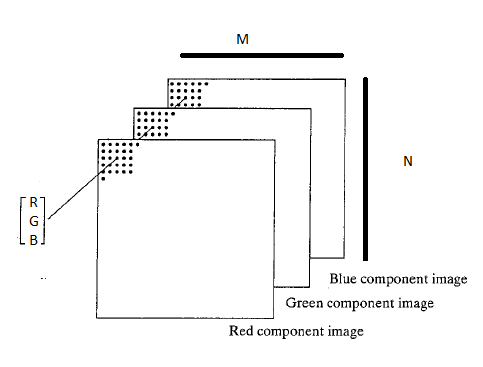
\includegraphics[scale=0.65]{fig/ImagenRGB.png}
	\caption{RGB Image}
	\label{fig:ImagenRGB}
\end{figure}

\subsection{Histogramas}

A partir de la imagen RGB se define la función  \emph{histograma}, la cual corresponde a la distribución de frecuencia de los valores que puede tomar una imagen $f$, ya sea en un plano o en 3 dimensiones (R, G, B). Se diferencian los siguientes tipos de histograma:

\subsubsection{Histograma de un componente}

El histograma del j-ésimo componente de la imagen a color $f$ (R, G o B) es una funci\'on discreta $h_{f_j}^{D}$ definida como:% $h:\{0,1,\dots,t_{max}\}\times \{C_1,C_2,\dots,C_n\}\rightarrow \mathbb N$ definida como:

\begin{equation}
\label{histograma}
   h_{f_j}^{D}(i) = n_i,
\end{equation} 
donde ${i}$ representa el $i-esimo$ nivel de intensidad en el rango $\{0,1,...,2^k-1\}$ del componente $j$, y $n_i$ es el n\'umero de pixeles en la imagen $f$ cuyo nivel de intensidad es $i$ en el componente $j$ dentro del dominio $D$ (subconjunto de pixeles $(u,v)$ dentro de la imagen $f$).

La probabilidad de aparici\'on $p_{f_j}^{D}(i)$ de cada nivel de intensidad $i$ en el componente $j$ de la imagen $f$ dentro del dominio $D$ es definida como:
\begin{equation}
\label{probabilidad}
   p_{f_j}^{D}(i) = \frac{h_{f_j}^{D}(i)}{n},
\end{equation} Donde $n = n_0 + n_1 + ... + n_{255}$, es decir la cantidad total de pixeles de la imagen $f$ dentro del dominio $D$. 

\subsubsection{Histograma de color}
El histograma a color  de una imagen $f $ en un dominio $D$  es una función discreta definida como sigue:
	
	\begin{equation}
	\label{eq:histograma_color}
	H^D_{f}(C) = n_C,
	\end{equation} donde  $C = (C_1, C_2, C_3)$, $C_i \in \{0, ..., 2^k - 1\}$ y $n_C$ es la cantidad de veces que aparece el color $C$ en el dominio $D$ de la imagen $f$. 
	
	Etiquetemos a cada color dentro del espacio discreto con los superíndices $a$  y $b$. El color $C^a$  es menor al color $C^b$ si $C^a_1 < C^b_1$, $C^a_2 < C^b_2$ y  $C^a_3 < C^b_3$. 
	
	El objetivo es fijar un orden de colores en el espacio de color discreto, normalmente utilizando el orden natural ascendente (Cuadro \ref{table:orden_color}).
	
	\begin{table}[!htpb]
		\centering
		\caption{Orden natural de colores}
		\label{table:orden_color}
		\begin{tabular}{|c|c|}
			\hline
			$a$   & $C^a$                                                                     \\ \hline
			0   & (0, 0, 0)                                                             \\ \hline
			1   & (0, 0, 1)                                                             \\ \hline
			2   & (0, 0, 2)                                                             \\ \hline
			3   & (0, 0, 3)                                                             \\ \hline
			\vdots & \vdots                                                                      \\ \hline
			$2^{3k}-2$ & ($2^k-2$, $2^k-2$, $2^k-2$) \\ \hline
			$2^{3k}-1$   & ($2^k-1$, $2^k-1$, $2^k-1$) \\ \hline
		\end{tabular}
	\end{table}
	
	El histograma de color acumulado $\bar{H}^D_f$ de la imagen $f$ un dominio $D$ es definido en términos del histograma a color $H^D_{f}$: 
	
	\begin{equation}
	\bar{H}^D_f(C^b) = \sum_{C^a \leq C^b} H^D_f(C^a)
	\end{equation}


El filtrado de im\'agenes abarca todas las t\'ecnicas dentro del procesamiento de im\'agenes, que a partir de una imagen de entrada, se obtenga otra imagen donde se elimine, se enfatice o resalte algunas caracter\'isticas de la imagen de entrada. A continuaci\'on se explicar\'a brevemente en que consiste el filtrado de im\'agenes a color. 

\subsection{Filtrado  de im\'agenes}
Un filtro $F$ de una imagen digital a color $f$ se puede expresar como:

\begin{equation}
\label{Filtrado} 
      g(u,v) = F\{f(u,v)\}
\end{equation}
donde $f(u,v)$ es un color de la imagen de entrada, $g(u,v)$ es un color de la imagen de salida y $F$ es el filtro definido sobre una ventana del pixel $(u,v)$.


Los filtros de orden son operaciones de vecindad no lineal, donde una funci\'on es aplicada al vecindario de cada pixel. La idea es mover una ventana centrada en el pixel, ya sea un rectangulo (usualmente un rectangulo con lados impares) o otra forma sobre una imagen dada. Al hacer esto, creamos una nueva imagen cuyo p\'ixeles son el resultado de obtener un valor de los los colores bajo la m\'ascara previamente ordenados (Figura \ref{fig:Filt}). 


\begin{figure}[htbp]
	\centering
		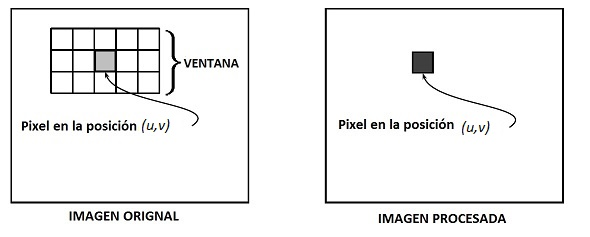
\includegraphics[scale=0.5]{fig/Filt.jpg}
	\caption{Filtrado de la imagen digital.}
	\label{fig:Filt}
\end{figure}



Por ejemplo un pixel de la nueva imagen puede ser resultado de obtener la mediana, el m\'inimo o m\'aximo de los colores ordenados en la ventana de la imagen procesada.  
La combinaci\'on de la ventana y la funci\'on es llamada filtro. 

 \subsection{Matem\'atica morfol\'ogica}

La extensi\'on de la matem\'atica morfol\'ogica imágenes a color es todav\'ia un problema abierto \cite{aptoula2007pseudo}, principalmente por el incoveniente de que no existe un orden natural entre los vectores, y que los colores pueden representarse de diversas formas (formando distintos espacios de color). Los operadores b\'asicos de erosi\'on y dilataci\'on se pueden definir a partir del m\'inimo y el m\'aximo dentro de una ventana llamada elemento estructurante. A partir de la erosi\'on y la dilataci\'on se puede extender toda la matem\'atica morfol\'ogica. De manera te\'orica los operadores morfol\'ogicos deben de cumplir ciertas propiedades, como ser anti-extensivo o extensivo, idempotentes, homot\'opicos y crecientes \cite{serra1986introduction}.

Dada una imagen digital $f$ y una ventana $B$, llamada elemento estructurante. La erosi\'on ($\varepsilon$) y la dilataci\'on ($\delta$) de la imagen $f$ por $B$ puede expresarse como:

\begin{equation}
\varepsilon(f,B)(u,v)  = \min_{(s,t) \in B} \{f(u-s,v-t) + B(s,t) \}
\end{equation}

\begin{equation}
\delta(f,B)(u,v)  =  \max_{(s,t) \in B} \{f(u+s,v+t) - B(s,t) \}
\end{equation}

Denotamos $\delta(f,B)$ y $\varepsilon(f,B)$ como la dilataci\'on y la erosi\'on respectivamente para todos los pixeles $(u,v)$ de la imagen $f$.

La apertura $\circ$ y el cierre $\bullet$ de $f$ por $B$ son definidas basadas en dilataci\'on y erosi\'on como sigue:

\begin{equation}
f\circ B = \delta(\varepsilon(f,B),B),
\end{equation}

\begin{equation}
f\bullet B = \varepsilon(\delta(f,B),B).
\end{equation}

Basado en la apertura y el cierre, la transformada top-hat, incluyendo la transformada top-hat clara ($WTH$) y la transformada top-hat oscura ($BTH$)  de la imagen $f$ son definidas como sigue:

\begin{equation}
WTH(f) = f - f\circ B,
\end{equation}

\begin{equation}
BTH(f) = f\bullet B - f. 
\end{equation}

La apertura suaviza las regiones brillantes de la imagen. El cierre suaviza las zonas oscuras de la imagen. Luego, $WTH$ podr\'ia extraer regiones brillantes de la imagen, mientras que $BTH$ podr\'ia extraer zonas oscuras.


\subsection{Ordenamiento}
El concepto de orden juega un rol fundamental para utilizar un filtro de orden, o poder definir las operaciones b\'asicas de la matem\'atica morfol\'ogica. Para un estudio profundo de la teor\'ia de orden el lector puede ver \cite{serra1993anamorphoses}.

%Una relaci\'on binaria $\leq$ en un dominio $D$ se llama:

%\begin{enumerate}
%\item \label{reflexiva} reflexiva si $C\leq C'$, $\forall C\in D$		 
%\item \label{antisimetrica} antisim\'etrica si $C \leq C' \wedge C' \leq C$\,$\Rightarrow$ \, $C=C'$,  $\forall C,C'\in D$
%\item \label{transitiva} transitiva si $C \leq C'$ $\wedge$ $C' \leq C''$\,$\Rightarrow$ \, $C \leq C''$,  $\forall C,C',C''\in D$
%\item \label{total} total si $C' \leq C$ $\vee$ $C' \leq C$,  $\forall C,C'\in D$
%\end{enumerate}
%Una relaci\'on binaria $\leq$ es llamada de \emph{pre-orden} si cumple con \ref{reflexiva} y \ref{transitiva}; si a su vez cumple con \ref{antisimetrica} se convierte en una relaci\'on de \emph{orden}. Si adicionalmente cumple con \ref{total}, es denotada como \emph{total}, si no lo hace como \emph{parcial}.
  
%La estructura en un espacio de color est\'a dada por un ret\'iculo completo. Un ret\'iculo completo ${\cal L}$ es un conjunto no vac\'io con orden parcial  ${\cal R} $ tal que cualquier subconjunto no vac\'io  ${\cal P}$ de  ${\cal L}$ tiene un \'infimo  y tiene un supremo. 

De acuerdo con el art\'iculo \cite{barnett1976ordering} las t\'ecnicas de ordenamiento vectorial se pueden clasificar en los siguientes grupos:
\begin{itemize}
\item Ordenamiento marginal (Ordenamiento M): El ordenamiento marginal compara cada componente del color de manera independiente.
\item Ordenamiento condicional (Ordenamiento C): Los vectores son ordenados por medio de algun componente marginal, seleccionado secuencialmente de acuerdo con diferentes condiciones. El orden lexicogr\'afico es un ejemplo bastante conocido de Ordenamiento C que emplea todos los componentes disponibles de los vectores dados.
\item Ordenamiento Parcial (Ordenamiento P): Este ordenamiento est\'a basado en la partici\'on de los vectores en grupos de equivalencia, tal que entre los grupos existe un orden. En este caso, ``parcial'' es un abuso de terminolog\'ia, ya que hay ordenamientos totales que pertenecen a esta clase en particular. 
\item Ordenamiento Reducido (Ordenamiento R): Los vectores se reducen primeramente a valores escalares y luego clasificados de acuerdo a su orden escalar natural. Por ejemplo, un ordenamiento R en $\mathbb{Z}^n$ podr\'ia consistir en definir primero una transformaci\'on $T:\mathbb{Z}^n\rightarrow \mathbb{R}$ y luego ordenar los colores con respecto al orden escalar de su proyecci\'on en $\mathbb{Z}^n$ por $T$.
\end{itemize}



 En la pr\'actica hay dos m\'etodos generales de procesamiento para im\'agenes a color: marginal y vectorial.

\subsubsection{Procesamiento marginal}
Consiste en el procesamiento por separado de cada componente de la imagen. A pesar de su sencillez, el procesamiento marginal tiene dos desventajas \cite{aptoula2007comparative}: 
\begin{itemize}
    \item La correlaci\'on entre los componentes es totalmente ignorado.
    \item Crea falsos colores despu\'es de su procesamiento.
\end{itemize}

La utilizaci\'on del procesamiento marginal es inadecuado para im\'agenes con componentes altamente correlacionados (por ejemplo, im\'agenes de color RGB) \cite{astola1990vector}. Por tal motivo este trabajo se concentrar\'a en el procesamiento vectorial que se explicar\'a a continuaci\'on. 

%\begin{figure}
%	\centering
%		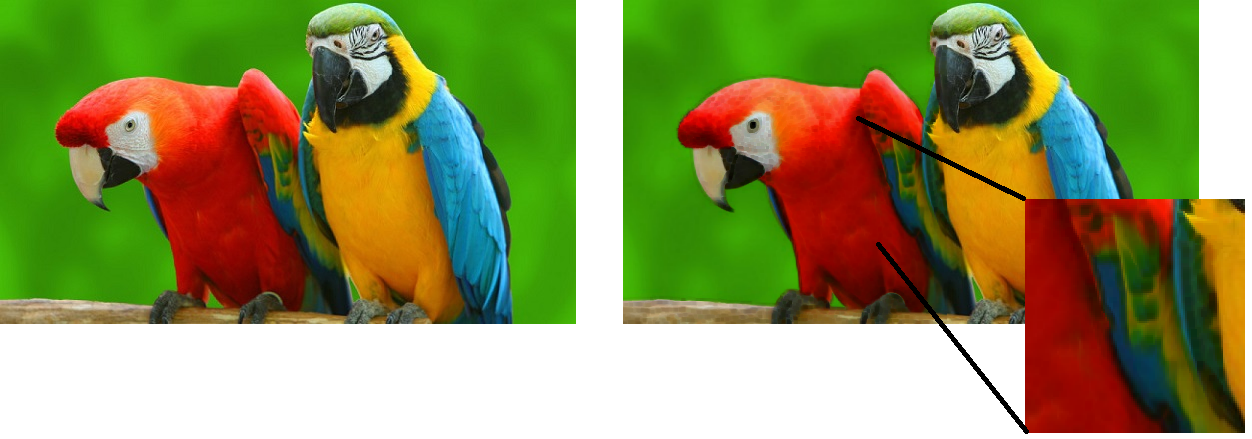
\includegraphics[scale=0.5]{fig/resultado.png}
%		\caption{Imagen original y su erosión utilizando el ordenamiento marginal. En la erosión aparecen %nuevas cromaticidades.}
%	\label{fig:resultado}
%\end{figure}


\subsubsection{Procesamiento vectorial}

Como su nombre lo indica, procesa todos los componentes disponibles globalmente y de forma simult\'anea.
Dado que los vectores (forma en que se representa un color) son considerados como los nuevas unidades de procesamiento, la correlaci\'on entre los diferentes componentes ya no es ignorada. Sin embargo, en comparaci\'on con su contraparte marginal, el inconveniente m\'as importante del enfoque vectorial es principalmente la necesidad de adaptar los algoritmos existentes con el fin de acomodar a datos vectoriales \cite{aptoula2007comparative}. 


El procesamiento vectorial puede tener dos enfoques:
 
\begin{itemize}
    \item El enfoque basado en relaci\'on de pre-orden.
    \item El enfoque basado en relaci\'on de orden.
\end{itemize}

El enfoque basado en relaci\'on de pre-orden, es el conjunto de enfoques que no cumplen la propiedad antisim\'etrica.  As\'i colores distintos eventualmente pueden llegar a ser equivalentes. De manera a resolver las ambiguedades existentes, es necesario medidas adicionales. El m\'etodo principal de ordenamiento de este enfoque est\'a basado en el Ordenamiento Reducido (Ordenamiento R), donde los colores son reducidos a valores escalares correspondientes a su norma, o distancia a alg\'un color de referencia. 


El enfoque basado en relaci\'on de orden, a su vez puede ser parcial o total. Si la relaci\'on es parcial, existir\'an colores que no podr\'an ser comparados. 

La relaci\'on de orden total presenta dos principales ventajas. Primero, todos los colores son comparables, y segundo, no existen colores distintos que pueden ser equivalentes. Debido a esto, la mayor\'ia de los trabajos est\'an basados en enfoques de relaci\'on de orden total \cite{aptoula2007comparative}. En particular, el orden lexicogr\'afico (Ordenamiento C), junto con sus variantes se encuentra entre las opciones m\'as implementadas.  

En la siguiente secci\'on se presenta una estrategia de ordenamiento de colores RGB, teniendo en cuenta m\'etricas extraidas de cada componente de color, de manera a establecer ponderaciones de los componentes a partir de informaci\'on propia de la imagen.



 \section{Ordenamiento propuesto}

De manera a evitar darle la mayor prioridad a un componente del vector que representa el color, se ubica un nuevo valor en la primera posici\'on de la cascada lexicogr\'afica correspondiente a una transformaci\'on obtenida a partir de m\'etricas asociadas a cada componente $(R,G,B)$.
Los colores RGB son reducidos a un valor escalar. Para tal efecto, se define primero una transformaci\'on $T:\mathbb{Z}^3 \rightarrow \mathbb{R}$ y luego se ordena los colores con respecto al orden escalar de su proyecci\'on en $\mathbb{Z}^3$ por $T$.
La reducci\'on de un color $
C=(C_1,C_2,C_3)$ se consigue por medio del producto interno del color $C$ con un vector de pesos $w=(w_1,w_2,w_3) $, es decir:

\begin{equation}
\label{Transformacion}
T(C)= \sum_{l=1}^3(w_l \cdot C_l)
\end{equation}  
donde $l$ es el \'indice del componente del color $C$ y $w_l \in \mathbb{R}$. 

Dos colores, $C=(C_1,C_2,C_3)$ e $C'=(C_1^{'},C_2^{'},C_3^{'})$, con $C\neq C'$, pueden tener la misma transformaci\'on, es decir $T(C) = T(C')$.  Por lo tanto, la transformaci\'on se utiliza como primer componente del orden lexicogr\'afico:

\begin{equation}
\label{Mio} 
 C\leq C'\Leftrightarrow [T(C),C_1,C_2,C_3] \leq_L [T(C'),C_1^{'},C_2^{'},C_3^{'}]
\end{equation} donde $\leq_L$ indica la relación $\leq$ según el orden lexicográfico.	

Oportunamente, despu\'es de la transformaci\'on se podr\'ia variar el orden de prioridad de los componentes de color.
Los valores del vector $w$ son obtenidos de aplicar una funci\'on $\phi \in \mathbb{R}$ sobre el histograma de cada componente en un dominio $D$ de la imagen $f$, es decir $w_1 = \phi(h_{f_1}^D)$, $w_2 = \phi(h_{f_2}^D)$, $w_3 = \phi(h_{f_3}^D)$, con $f_1$ = componente $R$, $f_2$ = componente $G$ y $f_3$ =  componente $B$.

La funci\'on $\phi$ puede ser obtenida a tr\'aves de aplicarle cualquier m\'etrica (por ejemplo estad\'istica) al histograma de cada componente  $(R,G,B)$, de manera de darle mayor peso a aquel componente cuya m\'etrica tenga mayor valor en un dominio $D$ espec\'ifico (puede ser toda la imagen o parte de la misma). 

 \section{Resultados experimentales}
En esta secci\'on se llevar\'a a cabo una serie de pruebas comparativas, con el fin de medir los rendimientos relativos de diferentes m\'etodos de ordenamiento del estado del arte junto al  ordenamiento propuesto, en tres aplicaciones de procesamiento de im\'agenes. Las aplicaciones seleccionadas fueron la eliminaci\'on de ruido, estiramiento de contraste y caracterización texturas para su posterior clasificación.
M\'as precisamente los m\'etodos de ordenamiento que participaron de las diferentes pruebas fueron:
el ordenamiento lexicogr\'afico cl\'asico, el ordenamiento $\alpha$-lexicogr\'afico \cite{zamora2001comparative}, el ordenamiento $\alpha$-modulo lexicogr\'afico \cite{angulo2003morphological}, ordenamiento lexicogr\'afico en el espacio HSI, comparando primero la I, luego la S, y por último la H (propuesto en \cite{ortiz2004gaussian}), la distancia euclidiana al color $(0,0,0)$ en el espacio de color L*a*b* y RGB \cite{ortiz2002procesamiento}, y el entrelazado de bits \cite{chanussot1997bit}. 
Todas las im\'agenes utilizadas en las diferentes pruebas fueron de $8$ bits. 

La funci\'on $\phi$ aplicada al histograma de cada componente $j$ de la imagen $f$ en todas las pruebas son:

\begin{itemize}
    \item Promedio ($Me$): Es la sumatoria de todos los niveles de intensidades $i$ que aparecen en el dominio $D$ sobre la cantidad total $n$ de pixeles que se encuentran en $D$:
		
\begin{equation}
\label{promedio}
   Me(h_{f_j}^D) = \sum_{i=0}^{255}\frac{i\times h_{f_j}^D(i)}{n},
\end{equation}		
Donde $n = n_0 + n_1 + ... + n_{255}$.

    \item M\'inimo($Min$): es el menor nivel de intensidad $i$ en el dominio $D$:
\begin{equation}
\label{minimo}
	Min(h_{f_j}^D) = \min\{i|h_{f_j}^D(i)>0\}
\end{equation}		
		\item M\'aximo($Max$): es el mayor nivel de intensidad $i$ en el dominio $D$:
\begin{equation}
\label{maximo}
   Max(h_{f_j}^D) = \max\{i|h_{f_j}^D(i)>0\}
\end{equation}		
 		\item Moda Minimo ($minM_o$): es el menor nivel de intensidad $i$ que aparece m\'as veces en el dominio $D$, es decir el menor nivel de intensidad $i$ que tiene mayor $p_{C}^D(i)$:
\begin{equation}
\label{ModaMinimo}
   minM_o(h_{f_j}^D) = \min\{i|h_{f_j}^D(i) \geq h_{f_j}^D(i'), \forall i\neq i'\}
\end{equation}		
\item Moda M\'aximo ($maxM_o$): es el mayor nivel de intensidad $i$ que aparece m\'as veces en el dominio $D$, es decir el mayor nivel de intensidad $i$ que tiene mayor $p_{C}^D(i)$:
\begin{equation}
\label{ModaMinimo}
   maxM_o(h_{f_j}^D) = \max\{i|h_{f_j}^D(i) \geq h_{f_j}^D(i'), \forall i\neq i'\}
\end{equation}				
    
		
		\item Varianza ($Var$): es la varianza de los niveles de intensidad $i$ en el dominio $D$:
  \begin{equation}
\label{varianza}
   Var(h_{f_j}^D) = \sum_{i=0}^{255}\frac{h_{f_j}^D(i)\times(i - Me(h_{f_j}^D))^2}{n}
\end{equation}		
		\item Suavidad($R$): Medida de suavidad relativa de la intensidad en el dominio $D$:
 \begin{equation}
\label{Suavidad}
   R(h_{f_j}^D) = 1-\frac{1}{1+Var(h_{f_j}^D)}
\end{equation}		
		

\end{itemize}


Un par\'ametro a ser definido es el dominio a ser tenido en cuenta para el c\'alculo
de los pesos $w_l$. Las distribuciones de dominio que fueron empleadas para las diferentes aplicaciones son explicadas a continuaci\'on.

\subsection{Vecindario como Dominio}


El dominio $D$ donde se aplica la funci\'on $\phi$ aplicada al histograma de cada componente $h_{f_j}^D$ es la propia ventana $B$ (llamado elemento estructurante para matem\'atica morfol\'ologica) donde se hace la operaci\'on del filtro no lineal. En la Figura \ref{fig:Ventana B} se puede observar un dominio $D$ correspondiente a un vecindario $B$ de tama\~no 3 $\times$ 3 centrado en el pixel $(u,v)$.

\begin{figure}
	\centering
		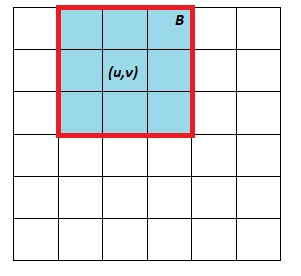
\includegraphics[width=0.3\textwidth]{fig/VentanaB.jpg}
	\caption{Vecindario $B$ de tama\~no 3 $\times$ 3 centrado en el pixel $(u,v)$ }
	\label{fig:Ventana B}
\end{figure}

\subsection{Divisi\'on de la imagen en sub-regiones}

La imagen $f$ se divide en sub-regiones $W_1,W_2,\dots W_{x}$, de manera a obtener informaci\'on local de  la imagen. 

Sea $B$ una ventana o  elemento estructurante, el dominio $D$ correspondiente a la ventana $B$ centrada en $(u,v)$ es el conjunto de sub-regiones $W_{\{1,2,...,x\}}$, que tocan alg\'un pixel de $B$.
%\begin{equation}
%\label{ventana}
%  \forall i, W_i \subseteq D_{(u,v)}\rightarrow \exists  \in D_{(u,v)}:x \in W_i
%\end{equation}   

En la Figura \ref{fig:Sub-region} la imagen se divide en 4 sub-regiones: $W_1$, $W_2$, $W_3$, $W_4$.

%\begin{figure}
%	\centering
%		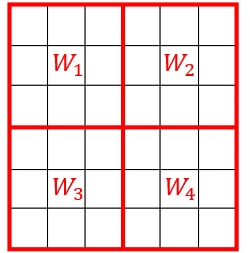
\includegraphics{fig/ventanas.png}
%	\caption{Imagen divida en 4 sub-regiones}
%	\label{fig:ventanas}
%\end{figure}


 La regi\'on delimitada por la ventana $B$ se encuentra sombreada. Como puede verse, el dominio
$D$ sobre el cual se calcular\'an los pesos $w_l$ para $B$ ser\'a la zona correspondiente a la
sub-region $W_1$. Cabe destacar que la ventana del filtro no tiene por qu\'e ser de igual
tama\~no que las sub-regiones, como en este caso.


\begin{figure}
	\centering
		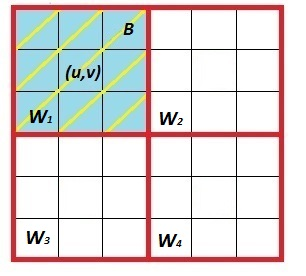
\includegraphics[width=0.3\textwidth]{fig/Sub-region.jpg}
	\caption{Dominio cuando la ventana toca una sub-regi\'on}
	\label{fig:Sub-region}
\end{figure}

En la Figura \ref{fig:Sub-regiones} se puede observar como el dominio $D$ de donde se calcular\'an los pesos pertenece a la uni\'on de las sub-regiones $W_1$ y $W_2$, ya que la ventana $B$ toca ambas. Esto se realiza para evitar que en el momento de la comparaci\'on dos colores  iguales puedan tener distintos valores, afectados por los pesos que vengan de dos sub-regiones distintas.  


\begin{figure}
	\centering
		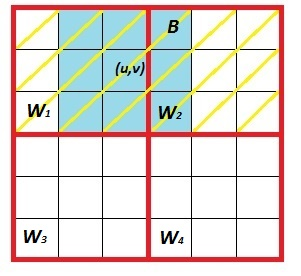
\includegraphics[width=0.3\textwidth]{fig/Sub-regiones.jpg}
	\caption{Dominio cuando la ventana toca m\'as de una sub-regi\'on.}
	\label{fig:Sub-regiones}
\end{figure} En el caso que el usuario solo seleccione tener una sub-regi\'on, es decir no dividir la imagen $f$, los pesos ser\'an calculados teniendo en cuenta toda la imagen $f$ como dominio $D$. 

En nuestros pruebas, las im\'agenes de entradas de tama\~no $M \times N$ pixeles, son divididas en sub-regiones $W_{\{1,2,...,x\}}$ de $M \times N$ pixeles, de $\left\lfloor\frac{M}{M'}\right\rfloor$ filas y $\left\lfloor\frac{N}{N'}\right\rfloor$ columnas, donde $\left\lfloor.\right\rfloor$ denota la funci\'on piso. De esta forma, una nueva matriz de $M'$ filas y $N'$ columnas, cuyo elemento es una sub-region $W_l$.



\subsection{Aplicaci\'on 1: Eliminaci\'on de ruido}
Ruido es un t\'ermino utilizado para denominar a las modificaciones indeseadas que puede sufrir una se\~nal de cualquier naturaleza durante su captura, almacenamiento, transmisi\'on, procesamiento o conversi\'on \cite{tuzlukov2002signal}.

El ruido en im\'agenes es un producto indeseable que agrega informaci\'on err\'onea y ajena a las mismas. El ruido se presenta en las im\'agenes digitales en forma de variaciones aleatorias en el brillo o informaci\'on de color. 
Varios modelos matem\'aticos han sido desarrollados de modo a simular la generaci\'on de los distintos 
tipos de ruido existentes. 
\subsubsection{Ruidos Utilizados}

Los principales modelos de ruidos y utilizados en las pruebas de este trabajo son \cite{davenport1958random}:

\begin{itemize}
	\item Ruido gaussiano: es un ruido estad\'istico aditivo con funci\'on de densidad de probabilidad gaussiana.
	\item Ruido speckle: es un ruido multiplicativo con funci\'on de densidad de probabilidad uniforme.
	\item Ruido sal y pimienta: no es un ruido aditivo ni multiplicativo con respecto a los valores de la imagen original. Los valores originales son reemplazados por valores brillantes (sal) u oscuros (pimienta), que corresponden a impulsos dentro de la se\~nal. 
\end{itemize}
En la Figura \ref{fig:ruido}(a) se puede observar una imagen que es contaminada con ruido gaussiano ( \ref{fig:ruido}(b)), ruido speckle (\ref{fig:ruido}(c)), con ruido sal y pimienta (\ref{fig:ruido}(d)). 

%\begin{figure}[htbp]
%\centering
%\subfigure[Imagen original]{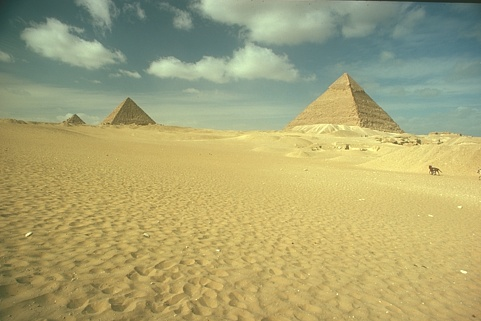
\includegraphics[width=73mm]{fig/Original_SinRuido.jpg}}
%\subfigure[Imagen con ruido gaussiano ($\sigma^2 = 0.05, \mu=0$)]{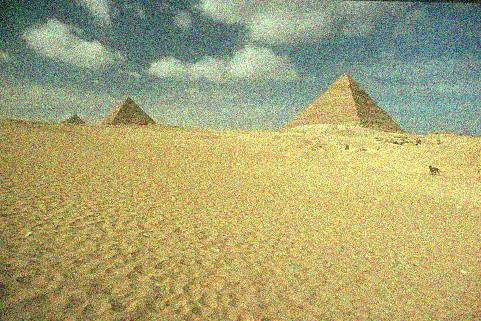
\includegraphics[width=73mm]{fig/img_gaussian_noise.jpg}}
%\subfigure[Imagen con ruido speckle ($\sigma^2 = 0.05, \mu=0$)]{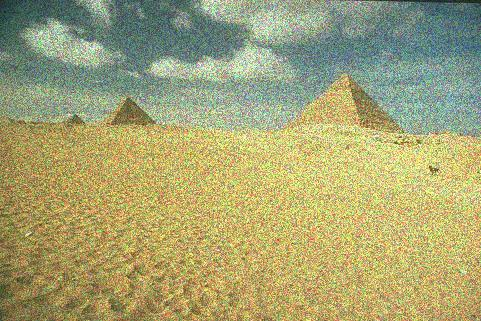
\includegraphics[width=73mm]{fig/img_speckle_noise.jpg}}
%\subfigure[Imagen con ruido sal y pimienta ($p = 0.05$)]{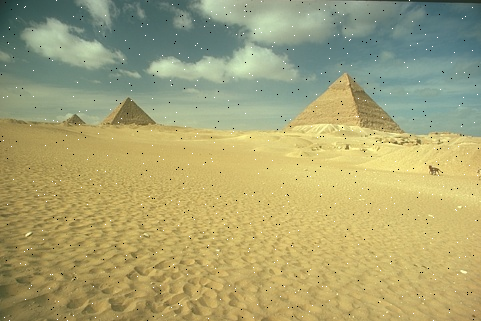
\includegraphics[width=73mm]{fig/img_salt_and_pepper_noise.jpg}}
%\caption{Imagen con diferentes tipos de ruidos.} \label{fig:ruido}
%\end{figure}


\begin{figure*}
	\makebox[\linewidth][c]{%
		\begin{subfigure}[b]{0.4\textwidth}
			\centering
			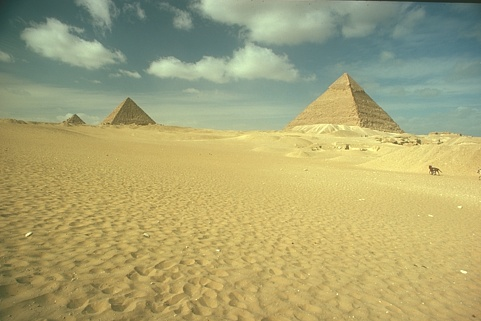
\includegraphics[width=0.95\textwidth]{fig/Original_SinRuido.jpg}
			\caption{Imagen original}
			\label{fig:original_sin_ruido}
		\end{subfigure}
		\begin{subfigure}[b]{0.4\textwidth}
			\centering
			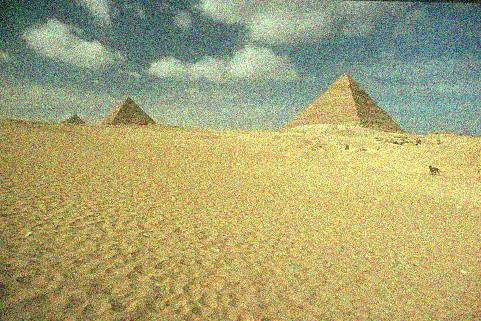
\includegraphics[width=0.95\textwidth]{fig/img_gaussian_noise.jpg}
			\caption{Imagen con ruido gaussiano ($\mu = 0; \sigma^2 = 0.05$)}
			\label{fig:con_ruido_gaussiano}
		\end{subfigure}
	}\\
	\makebox[\linewidth][c]{%
		\begin{subfigure}[b]{0.4\textwidth}
			\centering
			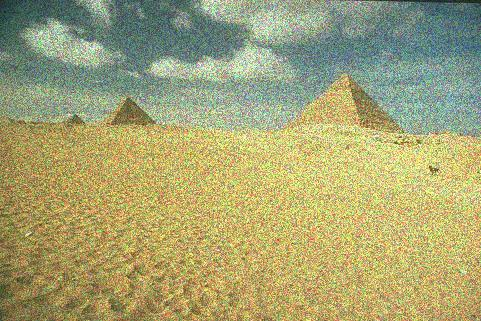
\includegraphics[width=0.95\textwidth]{fig/img_speckle_noise.jpg}
			\caption{Imagen con ruido speckle ($\mu = 0; \sigma^2 = 0.05$)}
			\label{fig:con_ruido_speckle}
		\end{subfigure}
			\begin{subfigure}[b]{0.4\textwidth}
				\centering
				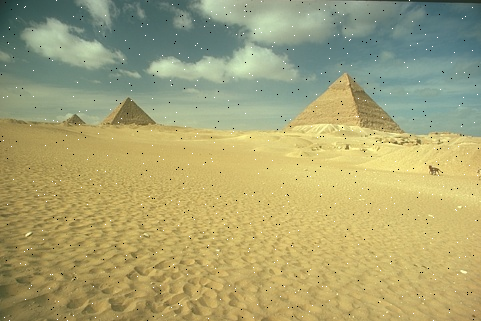
\includegraphics[width=0.95\textwidth]{fig/img_salt_and_pepper_noise.jpg}
				\caption{Imagen con ruido sal y pimienta ($p = 0.05$)}
				\label{fig:con_ruido_sal_y_pimienta}
			\end{subfigure}
	}\\
	\caption{Imagen con diferentes tipos de ruidos.} \label{fig:ruido}
\end{figure*}





%Los par\'ametros utilizados en la generaci\'on de cada ruido fueron:

%\begin{itemize}
%	\item Ruido gaussiano: La media  $\mu=0$ y  la varianza $\sigma^2$ fue variando  entre los valores 0,01 y 0,17, haciendo pasos de 0,01. 
%	\item Ruido speckle: La media  $\mu=0$ y  la varianza $\sigma^2$ fue variando  entre los valores 0,01 y 0,17, haciendo pasos de 0,01. 
%	\item Ruido sal y pimienta: El valor de probabilidad $p$  de ocurrencia de un ruido sal o pimienta fue variando  entre los valores 0,01 y 0,17, haciendo pasos de 0,01. 
%\end{itemize}

%El valor de la varianza $\sigma^2$ para los ruidos gaussiano y speckle, as\'i como el valor de probabilidad $p$ de ocurriencia de un ruido sal o pimienta fue variando  de manera a observar como se comporta el filtro a medida que se va aumentando la cantidad de ruido.


\subsubsection{M\'etricas Utilizadas}

En este apartado son detalladas las métricas MAE y CDS, las cuales fueron utilizadas para evaluar el desempeño de los distintos filtros utilizados para eliminación de ruido.

\textsl{MAE (Mean Absolute Error, Error Absoluto Promedio):} es una m\'etrica utilizada en estad\'istica para medir que tan cerca est\'an los pron\'osticos o predicciones de los resultados reales \cite{willmott2005advantages}. Dadas una imagen $f$ de dimensiones $M \times N$  y su imagen filtrada correspondiente $g$, el error absoluto promedio de la imagen filtrada est\'a dado por:
\begin{equation}
\label{MAE}
MAE(f,g) = \frac{1}{3}\sum_{j=1}^3 d_j
\end{equation} donde: 


\begin{equation}
d_j = \sum_{\substack{u\in \{1, ..., M\}\\ v \in \{1, ..., N\}}} |[f(u,v)]_{j} - [g(u,v)]_{j}| 
\end{equation}

La m\'etrica MAE resulta ser una m\'etrica de naturaleza marginal porque no tiene en cuenta a los vectores de colores como una unidad, sino que realiza el c\'alculo del error por componente y lo promedia.

De modo a validar el filtro se ha considerado la inclusi\'on de otra m\'etrica adem\'as de MAE, para evaluar los resultados desde una perspectiva vectorial, es decir, que procese a los colores como un conjunto.


\textsl{CDS (Color Distribution Similarity, Similaridad de Distribuciones de Color):} es una medida de similaridad para imágenes digitales a color basada en la diferencia de histogramas acumulados \cite{stricker1995similarity}.  La principal mejora de la diferencia de histogramas a color acumulado con respecto a la diferencia de histogramas a color radica; en que la diferencia de histograma a color acumulado obtiene todas las imágenes con similaridad perceptual a sus histogramas a color y de esta manera disminuye la probabilidad de obtener falsos negativos.

Para determinar la similaridad de dos imágenes $f$ y $g$, con histogramas acumulados a color $\bar{H}^D_f$ y $\bar{H}^D_g$ en un dominio $D$, se calcula la diferencia entre $\bar{H}^D_f$ y $\bar{H}^D_g$: 
\begin{equation}
CDS(f,g) = \sqrt{\sum_{\substack{u\in \{1, ..., M\}\\ v \in \{1, ..., N\}}} (\bar{H}^D_f(f(u, v)) - \bar{H}^D_g(g(u, v)))^2}
\end{equation}

%\include{anexos/graficos}
\subsubsection{Resultados}

A continuaci\'on se listan los c\'odigos utilizados para abreviar los nombres de los métodos de ordenamiento que fueron objeto de experimentación:


\begin{itemize}
	\item ED: Se utiliza la Distancia Euclidiana  RGB como m\'etodo de ordenamiento de los colores \cite{ortiz2002procesamiento}.
	\item BM: Se utiliza el Entrelazado de Bits RGB como m\'etodo de ordenamiento de los colores \cite{chanussot1997bit}.
	\item LEX: Se utiliza el ordenamiento lexicogr\'afico RGB para ordenar los colores .
	\item ALEX: Se utiliza el ordenamiento $\alpha$-lexicogr\'afico RGB \cite{zamora2001comparative} para ordenar los colores.
	\item AMLEX: Se utiliza el  $\alpha$-modulo lexicogr\'afico RGB \cite{angulo2003morphological} para ordenar los colores.
	\item HLEX, se utiliza el ordenamiento Lexicográfico HSI para ordenar los colores.
	\item DLAB, se utiliza la Distancia en L*a*b* como m\'etodo de ordenamiento \cite{ortiz2002procesamiento}.
	\item MIN: se utiliza la ecuaci\'on \ref{Transformacion} para agregar esta transformaci\'on como primer componente de la cascada lexicogr\'afica RGB, donde:\\ 
$w = (Min(h_{f_1}^D), Min(h_{f_2}^D),Min(h_{f_3}^D))$.
	\item MAX: se utiliza la ecuaci\'on \ref{Transformacion} para agregar esta transformaci\'on como primer componente de la cascada lexicogr\'afica RGB, donde:\\ 
$w = (Max(h_{f_1}^D), Max(h_{f_2}^D),Max(h_{f_3}^D))$.
	\item MO1: se utiliza la ecuaci\'on \ref{Transformacion} para agregar esta transformaci\'on como primer componente de la cascada lexicogr\'afica RGB, donde:\\ 
$w = (minM_o(h_{f_1}^D), minM_o(h_{f_2}^D), minM_o(h_{f_3}^D))$.
	\item MO2: se utiliza la ecuaci\'on \ref{Transformacion} para agregar esta transformaci\'on como primer componente de la cascada lexicogr\'afica RGB, donde:\\ 
$w = (maxM_o(h_{f_1}^D), maxM_o(h_{f_2}^D), maxM_o(h_{f_3}^D))$.
	\item SMO: se utiliza la ecuaci\'on \ref{Transformacion} para agregar esta transformaci\'on como primer componente de la cascada lexicogr\'afica RGB, donde:\\ 
$w = (R(h_{f_1}^D), R(h_{f_2}^D), R(h_{f_3}^D))$.
	\item MEAN: se utiliza la ecuaci\'on \ref{Transformacion} para agregar esta transformaci\'on como primer componente de la cascada lexicogr\'afica RGB, donde:\\ 
$w = (Me(h_{f_1}^D), Me(h_{f_2}^D), Me(h_{f_3}^D))$.
	\item VAR: se utiliza la ecuaci\'on \ref{Transformacion} para agregar esta transformaci\'on como primer componente de la cascada lexicogr\'afica RGB, donde:\\ 
$w = (Var(h_{f_1}^D), Var(h_{f_2}^D), Var(h_{f_3}^D))$.
\end{itemize}

El filtro utilizado para eliminar los diferentes tipos de ruido fue la mediana. Este filtro consiste en ordenar los colores dentro de la ventana del filtro, y seleccionar el valor del medio para remplazar en la imagen de salida. De manera a evitar tener un falso color, el tama\~no de la ventana del filtro suele ser impar (en nuestras pruebas de tamaño $3\times 3$). Las pruebas fueron realizadas con 100 im\'agenes diferentes (im\'agenes de prueba de \cite{arbelaez2007berkeley}), contaminándolas con los ruidos sal y pimienta, gaussiano y speckle. En el caso de los ruidos gaussiano y speckle se mantuvo el parámetro $\mu = 0$ y se varió el parámetro $\sigma^2$ entre $0.005$ y $0.165$, con incrementos de $0.02$. En el caso del ruido sal y pimienta, el parámetro de probabibilidad $p$ se varió con los mismos valores del parámetro $\sigma^2$ de los ruidos gaussiano y speckle.

La Figura \ref{fig:imagen_ejemplo_ruido_gaussiano} corresponde a la imagen original de la Figura \ref{fig:ruido} con $\sigma^2 = 0.105$ y $\mu = 0$. El resultado de aplicar los filtros de orden propuestos y el resto de los filtros evaluados sobre la imagen contaminada puede verse en la Figura \ref{fig:imagenes_resultado}.


\begin{figure}
	\centering
	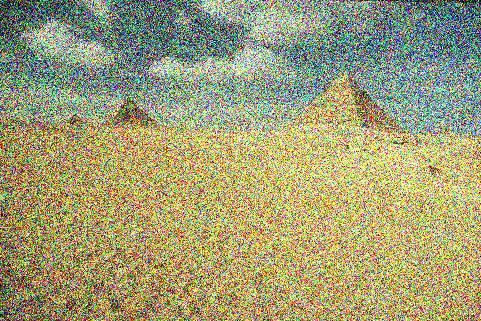
\includegraphics[width=0.38\textwidth]{fig/img_ruido_gaussian_83_0_105}
	\caption{Ruido gaussiano ($\mu = 0; \sigma^2 = 0.105$)}
	\label{fig:imagen_ejemplo_ruido_gaussiano}
\end{figure}


Cabe resaltar que las imágenes filtradas con el orden propuesto y con los diferentes pesos son mejores visualmente a los del estado del arte, pero son perceptualmente muy parecidas entre si, la diferencia entre ellas se evidencia en los resultados numéricos expuestos más adelante en esta sección.

\begin{figure*}
	\makebox[\linewidth][c]{%
		\begin{subfigure}[b]{0.25\textwidth}
			\centering
			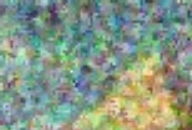
\includegraphics[width=0.95\linewidth]{fig/ALEX}
			\caption{ALEX}
			\label{fig:alex}
		\end{subfigure}
		\begin{subfigure}[b]{0.25\textwidth}
			\centering
			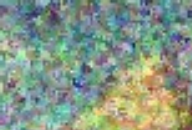
\includegraphics[width=0.95\linewidth]{fig/AMLEX}
			\caption{AMLEX}
			\label{fig:amlex}
		\end{subfigure}
		\begin{subfigure}[b]{0.25\textwidth}
			\centering
			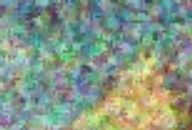
\includegraphics[width=0.95\linewidth]{fig/BM}
			\caption{BM}
			\label{fig:bm}
		\end{subfigure}
		\begin{subfigure}[b]{0.25\textwidth}
			\centering
			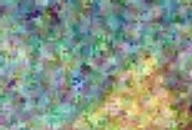
\includegraphics[width=0.95\linewidth]{fig/DLAB}
			\caption{DLAB}
			\label{fig:dlab}
		\end{subfigure}
	}\\
	\makebox[\linewidth][c]{%
		\begin{subfigure}[b]{0.25\textwidth}
			\centering
			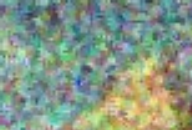
\includegraphics[width=0.95\linewidth]{fig/ED}
			\caption{ED}
			\label{fig:ed}
		\end{subfigure}
		\begin{subfigure}[b]{0.25\textwidth}
			\centering
			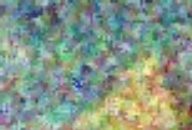
\includegraphics[width=0.95\linewidth]{fig/HLEX}
			\caption{HLEX}
			\label{fig:hlex}
			\phantomcaption
		\end{subfigure}
		\begin{subfigure}[b]{0.25\textwidth}
			\centering
			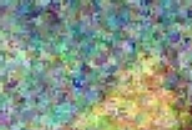
\includegraphics[width=0.95\linewidth]{fig/LEX}
			\caption{LEX}
			\label{fig:lex}
			\phantomcaption
		\end{subfigure}
		\begin{subfigure}[b]{0.25\textwidth}
			\centering
			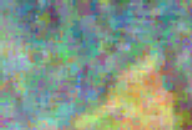
\includegraphics[width=0.95\linewidth]{fig/MAXM5}
			\caption{MAX}
			\label{fig:max}
			\phantomcaption
		\end{subfigure}
	}\\
	\makebox[\linewidth][c]{%
		\begin{subfigure}[b]{0.25\textwidth}
			\centering
			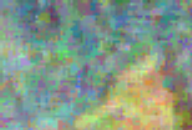
\includegraphics[width=0.95\linewidth]{fig/MEANM5}
			\caption{MEAN}
			\label{fig:mean}
			\phantomcaption
		\end{subfigure}
		\begin{subfigure}[b]{0.25\textwidth}
			\centering
			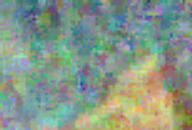
\includegraphics[width=0.95\linewidth]{fig/MINM5}
			\caption{MIN}
			\label{fig:min}
			\phantomcaption
		\end{subfigure}
		\begin{subfigure}[b]{0.25\textwidth}
			\centering
			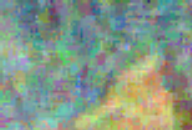
\includegraphics[width=0.95\linewidth]{fig/MOD2M5}
			\caption{MO2}
			\label{fig:mo2}
			\phantomcaption
		\end{subfigure}
		\begin{subfigure}[b]{0.25\textwidth}
			\centering
			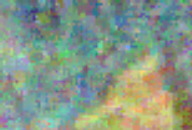
\includegraphics[width=0.95\linewidth]{fig/MODM5}
			\caption{MO1}
			\label{fig:mo1}
			\phantomcaption
		\end{subfigure}
	}\\
	\makebox[\linewidth][c]{%
		\begin{subfigure}[b]{0.25\textwidth}
			\centering
			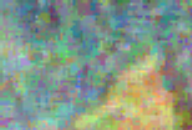
\includegraphics[width=0.95\linewidth]{fig/SMOM5}
			\caption{SMO}
			\label{fig:smo}
			\phantomcaption
		\end{subfigure}
		\begin{subfigure}[b]{0.25\textwidth}
			\centering
			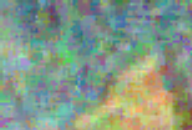
\includegraphics[width=0.95\linewidth]{fig/VARM5}
			\caption{VAR}
			\label{fig:var}
			\phantomcaption
		\end{subfigure}
	}\\
	\caption{Resultados de aplicar los distintos filtros evaluados sobre la imagen de la Figura \ref{fig:imagen_ejemplo_ruido_gaussiano}. La imagen fue divida en sub-regiones de 5 x 5.}	
	\label{fig:imagenes_resultado}
\end{figure*}

Por cada ruido y métrica se presenta una tabla de resultados y un gráfico de curvas de tendencia. Las tablas de resultados ordenan a los filtros según el promedio total que obtuvieron para todos los parámetros de ruido. Los filtros que aparecen en los primeros lugares de las tablas son aquellos que poseen los menores valores de área bajo la curva. En algunos casos, los filtros del estado del arte se comportan mejor para menores valores de parámetro de ruido pero se ven superados por los filtros propuestos para mayores valores de parámetro de ruido. 

Cada gráfico posee curvas de tendencia que representan a cada uno de los filtros evaluados. En el eje de ordenadas se ubican los valores de la métrica correspondiente (MAE y CDS). En el eje de abscisas se ubican los valores de parámetro de ruido variados. En una curva correspondiente a un filtro, cada punto representa al promedio de métrica obtenido por ese filtro para un cierto valor de parámetro de ruido.

Los resultados de esta sección diferencian a los filtros de orden de cada peso de acuerdo a su configuración de dominio. Como referencia, a los códigos de los filtros propuestos se les agrega el sufijo "WX", donde X es un número que representa la cantidad de sub-regiones en que fue dividida la imagen. Cuando el vecindario (marcado por la ventana del filtro) es el dominio, se utiliza el sufijo "W0".

%Para poder seleccionar varias columnas de una vez
\pgfplotstableset{
	my multistyler/.style 2 args={
		@my multistyler/.style={display columns/##1/.append style={#2}},
		@my multistyler/.list={#1}
	}
}

\pgfplotstableread[
col sep = tab,
header=has colnames,
]
{anexos/files/color_and_marker_by_filter.txt}{\colorbyfilter}



%mae gaussiano
\pgfplotstableread[
col sep = tab,
header=has colnames,
comment chars={P},
]
{anexos/files/ventanas_mae_gaussian.txt}{\ventanasmaegaussian}
\pgfplotstablegetcolsof{\ventanasmaegaussian}
\pgfmathsetmacro{\C}{\pgfplotsretval-1}
\pgfmathsetmacro{\B}{\C-1}
\pgfplotstablegetrowsof{\ventanasmaegaussian}
\pgfmathsetmacro{\R}{\pgfplotsretval -1}


\begin{figure*}
	\centering
	\begin{tikzpicture}[spy using outlines={circle, magnification=9.5, size=3.5cm, connect spies}]
	\begin{axis}[
	xmax = 0.175,
	legend style={mark options={scale=1.5}},
	xlabel={$\sigma^2$},
	ylabel={MAE},
	legend pos=outer north east,
	height=0.5\textwidth,
	width=0.6\textwidth,
	tick label style={/pgf/number format/fixed,
		/pgf/number format/precision=4}
	]
	\foreach \n in {\C,\B,...,1} {
		\pgfplotstablegetcolumnnamebyindex{\n}\of{\ventanasmaegaussian}\to{\colname}
		\pgfplotstablegetelem{0}{\colname}\of{\colorbyfilter}
		\let\color=\pgfplotsretval
		\pgfplotstablegetelem{1}{\colname}\of{\colorbyfilter}
		\let\marca=\pgfplotsretval
		\edef\temp{
			\noexpand\addplot+[\color, mark=\marca, solid, mark options={mark size = 1.5, fill=\color!70}] 
		}
		\temp	
		table[x=p, y index=\n]{\ventanasmaegaussian};
		
		\addlegendentryexpanded{\colname}
	}%
	\pgfplotstablegetelem{\R}{[index]1}\of{\ventanasmaegaussian}
	\let\ytozoom=\pgfplotsretval
	\coordinate (spypoint) at (axis cs:0.165,\ytozoom);
	\coordinate (spyviewer) at (axis cs:0.12,17);
	\spy on (spypoint) in node [fill=white] at (spyviewer);
	\end{axis}
	\end{tikzpicture}
	\caption{Ruido gaussiano. MAE por $\sigma^2$}
	\label{fig:gaussian_mae}
\end{figure*}
	

\begin{table*}
	\small
	\centering
	\caption{Ruido gaussiano. MAE por $\sigma^2$}
	\pgfkeys{/pgf/number format/precision=4}
	\pgfplotstabletypeset[
	col sep=tab,
	header=has colnames,
	every first column/.style={
		string type,
		column type/.add={|}{|},
%		postproc cell content/.append style={
%			/pgfplots/table/@cell content/.add={$\bf}{$},
%		},
	},
	every head row/.style={
		before row=\hline,
		after row=\hline
	},
	every last column/.style={column type/.add={}{|}},
	every last row/.style={
		after row=\hline,
	},
	every row 0 column 1/.style={
		postproc cell content/.style={
			@cell content/.add={$\bf}{$}
		}
	},
	every row 0 column 2/.style={
		postproc cell content/.style={
			@cell content/.add={$\bf}{$}
		}
	},
	every row 1 column 3/.style={
		postproc cell content/.style={
			@cell content/.add={$\bf}{$}
		}
	},
	every row 1 column 4/.style={
		postproc cell content/.style={
			@cell content/.add={$\bf}{$}
		}
	},
	every row 1 column 5/.style={
		postproc cell content/.style={
			@cell content/.add={$\bf}{$}
		}
	},
	every row 0 column 6/.style={
		postproc cell content/.style={
			@cell content/.add={$\bf}{$}
		}
	},
	every row 0 column 7/.style={
		postproc cell content/.style={
			@cell content/.add={$\bf}{$}
		}
	},
	every row 2 column 8/.style={
		postproc cell content/.style={
			@cell content/.add={$\bf}{$}
		}
	},
	every row 0 column 9/.style={
		postproc cell content/.style={
			@cell content/.add={$\bf}{$}
		}
	},
	]{anexos/files/ventanas_mae_gaussian_tabla.txt}
	\label{tabla:gaussian_mae}
\end{table*}

%mae sal y pimienta
\pgfplotstableread[
col sep = tab,
header=has colnames,
comment chars={P},
]
{anexos/files/ventanas_mae_salt_and_pepper.txt}{\ventanasmaesaltandpepper}


\begin{figure*}
	\centering
	\begin{tikzpicture}[spy using outlines={circle, magnification=9.5, size=3.5cm, connect spies}]
	\begin{axis}[
	xmax = 0.175,
	legend style={mark options={scale=1.5}},
	xlabel={$p$},
	ylabel={MAE},
	legend pos=outer north east,
	height=0.5\textwidth,
	width=0.6\textwidth,
	tick label style={/pgf/number format/fixed,
		/pgf/number format/precision=4}
	]
	\foreach \n in {\C,\B,...,1} {
		\pgfplotstablegetcolumnnamebyindex{\n}\of{\ventanasmaesaltandpepper}\to{\colname}
		\pgfplotstablegetelem{0}{\colname}\of{\colorbyfilter}
		\let\color=\pgfplotsretval
		\pgfplotstablegetelem{1}{\colname}\of{\colorbyfilter}
		\let\marca=\pgfplotsretval
		\edef\temp{
			\noexpand\addplot+[\color, mark=\marca, solid, mark options={mark size = 1.5, fill=\color!70}] 
		}
		\temp	
		table[x=p, y index=\n]{\ventanasmaesaltandpepper};
		
		\addlegendentryexpanded{\colname}	
	}%
	\pgfplotstablegetelem{\R}{[index]1}\of{\ventanasmaesaltandpepper}
	\let\ytozoom=\pgfplotsretval
	\coordinate (spypoint) at (axis cs:0.165,\ytozoom);
	\coordinate (spyviewer) at (axis cs:0.04,6.15);
	\spy on (spypoint) in node [fill=white] at (spyviewer);
	\end{axis}
	\end{tikzpicture}
	\caption{Ruido sal y pimienta. MAE por $p$}
	\label{fig:salt_and_pepper_mae}
\end{figure*}


\begin{table*}
	\small
	\centering
	\caption{Ruido sal y pimienta. MAE por $p$}
	\pgfkeys{/pgf/number format/precision=4}
	\pgfplotstabletypeset[
	col sep=tab,
	header=has colnames,
	every first column/.style={
		string type,
		column type/.add={|}{|},
	},
	every head row/.style={
		before row=\hline,
		after row=\hline
	},
	every last column/.style={column type/.add={}{|}},
	every last row/.style={
		after row=\hline,
	},
	every row 0 column 1/.style={
		postproc cell content/.style={
			@cell content/.add={$\bf}{$}
		}
	},
	every row 0 column 2/.style={
		postproc cell content/.style={
			@cell content/.add={$\bf}{$}
		}
	},
	every row 0 column 3/.style={
		postproc cell content/.style={
			@cell content/.add={$\bf}{$}
		}
	},
	every row 0 column 4/.style={
		postproc cell content/.style={
			@cell content/.add={$\bf}{$}
		}
	},
	every row 0 column 5/.style={
		postproc cell content/.style={
			@cell content/.add={$\bf}{$}
		}
	},
	every row 0 column 6/.style={
		postproc cell content/.style={
			@cell content/.add={$\bf}{$}
		}
	},
	every row 0 column 7/.style={
		postproc cell content/.style={
			@cell content/.add={$\bf}{$}
		}
	},
	every row 0 column 8/.style={
		postproc cell content/.style={
			@cell content/.add={$\bf}{$}
		}
	},
	every row 0 column 9/.style={
		postproc cell content/.style={
			@cell content/.add={$\bf}{$}
		}
	},
	]{anexos/files/ventanas_mae_salt_and_pepper_tabla.txt}
	\label{tabla:salt_and_pepper_mae}
\end{table*}

%mae speckle
\pgfplotstableread[
col sep = tab,
header=has colnames,
comment chars={P},
]
{anexos/files/ventanas_mae_speckle.txt}{\ventanasmaespeckle}
\pgfplotstablegetcolsof{\ventanasmaespeckle}
\pgfmathsetmacro{\C}{\pgfplotsretval-1}


\begin{figure*}
	\centering
	\begin{tikzpicture}[spy using outlines={circle, magnification=9.5, size=3.5cm, connect spies}]
	\begin{axis}[
	xmax = 0.175,
	legend style={mark options={scale=1.5}},
	xlabel={$p$},
	ylabel={MAE},
	legend pos=outer north east,
	height=0.5\textwidth,
	width=0.6\textwidth,
	tick label style={/pgf/number format/fixed,
		/pgf/number format/precision=4}
	]
	\foreach \n in {\C,\B,...,1} {
		\pgfplotstablegetcolumnnamebyindex{\n}\of{\ventanasmaespeckle}\to{\colname}
		\pgfplotstablegetelem{0}{\colname}\of{\colorbyfilter}
		\let\color=\pgfplotsretval
		\pgfplotstablegetelem{1}{\colname}\of{\colorbyfilter}
		\let\marca=\pgfplotsretval
		\edef\temp{
			\noexpand\addplot+[\color, mark=\marca, solid, mark options={mark size = 1.5, fill=\color!70}] 
		}
		\temp	
		table[x=p, y index=\n]{\ventanasmaespeckle};
		
		\addlegendentryexpanded{\colname}	
	}%
	\pgfplotstablegetelem{\R}{[index] 1}\of{\ventanasmaespeckle}
	\let\ytozoom=\pgfplotsretval
	\coordinate (spypoint) at (axis cs:0.165,\ytozoom);
	\coordinate (spyviewer) at (axis cs:0.12,13);
	\spy on (spypoint) in node [fill=white] at (spyviewer);
	\end{axis}
	\end{tikzpicture}
	\caption{Ruido speckle. MAE por $\sigma^2$}
	\label{fig:speckle_mae}
\end{figure*}


\begin{table*}
	\centering
	\small
	\caption{Ruido speckle. MAE por $\sigma^2$}
	\pgfkeys{/pgf/number format/precision=4}
	\pgfplotstabletypeset[
	col sep=tab,
	header=has colnames,
	every first column/.style={
		string type,
		column type/.add={|}{|},
	},
	every head row/.style={
		before row=\hline,
		after row=\hline
	},
	every last column/.style={column type/.add={}{|}},
	every last row/.style={
		after row=\hline,
	},
	every row 0 column 1/.style={
		postproc cell content/.style={
			@cell content/.add={$\bf}{$}
		}
	},
	every row 0 column 2/.style={
		postproc cell content/.style={
			@cell content/.add={$\bf}{$}
		}
	},
	every row 0 column 3/.style={
		postproc cell content/.style={
			@cell content/.add={$\bf}{$}
		}
	},
	every row 0 column 4/.style={
		postproc cell content/.style={
			@cell content/.add={$\bf}{$}
		}
	},
	every row 0 column 5/.style={
		postproc cell content/.style={
			@cell content/.add={$\bf}{$}
		}
	},
	every row 0 column 6/.style={
		postproc cell content/.style={
			@cell content/.add={$\bf}{$}
		}
	},
	every row 0 column 7/.style={
		postproc cell content/.style={
			@cell content/.add={$\bf}{$}
		}
	},
	every row 0 column 8/.style={
		postproc cell content/.style={
			@cell content/.add={$\bf}{$}
		}
	},
	every row 0 column 9/.style={
		postproc cell content/.style={
			@cell content/.add={$\bf}{$}
		}
	},
	]{anexos/files/ventanas_mae_speckle_tabla.txt}
	\label{tabla:speckle_mae}
\end{table*}

%cds gaussiano
\pgfplotstableread[
col sep = tab,
header=has colnames,
comment chars={P},
]
{anexos/files/ventanas_cds_gaussian.txt}{\ventanascdsgaussian}
\pgfplotstablegetcolsof{\ventanascdsgaussian}
\pgfmathsetmacro{\C}{\pgfplotsretval-1}


\begin{figure*}
	\centering
	\begin{tikzpicture}[spy using outlines={circle, magnification=9.5, size=3.5cm, connect spies}]
	\begin{axis}[
	xmax = 0.175,
	legend style={mark options={scale=1.5}},
	xlabel={$\sigma^2$},
	ylabel={CDS},
	legend pos=outer north east,
	height=0.5\textwidth,
	width=0.6\textwidth,
	tick label style={/pgf/number format/fixed,
		/pgf/number format/precision=4}
	]
	\foreach \n in {\C,\B,...,1} {
		\pgfplotstablegetcolumnnamebyindex{\n}\of{\ventanascdsgaussian}\to{\colname}
		\pgfplotstablegetelem{0}{\colname}\of{\colorbyfilter}
		\let\color=\pgfplotsretval
		\pgfplotstablegetelem{1}{\colname}\of{\colorbyfilter}
		\let\marca=\pgfplotsretval
		\edef\temp{
			\noexpand\addplot+[\color, mark=\marca, solid, mark options={mark size = 1.5, fill=\color!70}] 
		}
		\temp	
		table[x=p, y index=\n]{\ventanascdsgaussian};
		
		\addlegendentryexpanded{\colname}
	}%
	\pgfplotstablegetelem{\R}{[index]1}\of{\ventanascdsgaussian}
	\let\ytozoom=\pgfplotsretval
	\coordinate (spypoint) at (axis cs:0.165,\ytozoom);
	\coordinate (spyviewer) at (axis cs:0.1,22000000);
	\spy on (spypoint) in node [fill=white] at (spyviewer);
	\end{axis}
	\end{tikzpicture}
	\caption{Ruido gaussiano. CDS por $\sigma^2$}
	\label{fig:gaussian_cds}
\end{figure*}


\begin{table*}
	\small
	\centering
	\caption{Ruido gaussiano. $CDS \times 10^7$ por $\sigma^2$}
	\pgfkeys{/pgf/number format/precision=5}
	\pgfplotstabletypeset[
	col sep=tab,
	header=has colnames,
	every first column/.style={
		string type,
		column type/.add={|}{|}
	},
	every head row/.style={
		before row=\hline,
		after row=\hline
	},
	every last column/.style={column type/.add={}{|}},
	every last row/.style={
		after row=\hline,
	},
	every row 0 column 1/.style={
		postproc cell content/.style={
			@cell content/.add={$\bf}{$}
		}
	},
	every row 0 column 2/.style={
		postproc cell content/.style={
			@cell content/.add={$\bf}{$}
		}
	},
	every row 0 column 3/.style={
		postproc cell content/.style={
			@cell content/.add={$\bf}{$}
		}
	},
	every row 0 column 4/.style={
		postproc cell content/.style={
			@cell content/.add={$\bf}{$}
		}
	},
	every row 0 column 5/.style={
		postproc cell content/.style={
			@cell content/.add={$\bf}{$}
		}
	},
	every row 0 column 6/.style={
		postproc cell content/.style={
			@cell content/.add={$\bf}{$}
		}
	},
	every row 1 column 7/.style={
		postproc cell content/.style={
			@cell content/.add={$\bf}{$}
		}
	},
	every row 1 column 8/.style={
		postproc cell content/.style={
			@cell content/.add={$\bf}{$}
		}
	},
	every row 1 column 9/.style={
		postproc cell content/.style={
			@cell content/.add={$\bf}{$}
		}
	},
	my multistyler={1,...,17}{
		divide by={10000000}
	},
	]{anexos/files/ventanas_cds_gaussian_tabla.txt}
	\label{tabla:gaussian_cds}
\end{table*}

%cds sal y pimienta
\pgfplotstableread[
col sep = tab,
header=has colnames,
comment chars={P},
]
{anexos/files/ventanas_cds_salt_and_pepper.txt}{\ventanascdssaltandpepper}


\begin{figure*}
	\centering
	\begin{tikzpicture}[spy using outlines={circle, magnification=9.5, size=3.5cm, connect spies}]
	\begin{axis}[
	xmax = 0.175,
	legend style={mark options={scale=1.5}},
	xlabel={$p$},
	ylabel={CDS},
	legend pos=outer north east,
	height=0.5\textwidth,
	width=0.6\textwidth,
	tick label style={/pgf/number format/fixed,
		/pgf/number format/precision=4}
	]
	\foreach \n in {\C,\B,...,1} {
		\pgfplotstablegetcolumnnamebyindex{\n}\of{\ventanascdssaltandpepper}\to{\colname}
		\pgfplotstablegetelem{0}{\colname}\of{\colorbyfilter}
		\let\color=\pgfplotsretval
		\pgfplotstablegetelem{1}{\colname}\of{\colorbyfilter}
		\let\marca=\pgfplotsretval
		\edef\temp{
			\noexpand\addplot+[\color, mark=\marca, solid, mark options={mark size = 1.5, fill=\color!70}] 
		}
		\temp	
		table[x=p, y index=\n]{\ventanascdssaltandpepper};
		
		\addlegendentryexpanded{\colname}
	}%
	\pgfplotstablegetelem{\R}{MINW9}\of{\ventanascdssaltandpepper}
	\let\ytozoom=\pgfplotsretval
	\coordinate (spypoint) at (axis cs:0.165,\ytozoom);
	\coordinate (spyviewer) at (axis cs:0.137,10170000);
	\spy on (spypoint) in node [fill=white] at (spyviewer);
	\end{axis}
	\end{tikzpicture}
	\caption{Ruido sal y pimienta. CDS por $p$}
	\label{fig:salt_and_pepper_cds}
\end{figure*}


\begin{table*}
	\centering
	\small
	\caption{Ruido sal y pimienta. $CDS \times 10^7$ por $p$}
	\pgfkeys{/pgf/number format/precision=4}
	\pgfplotstabletypeset[
	col sep=tab,
	header=has colnames,
	every first column/.style={
		string type,
		column type/.add={|}{|},
	},
	every head row/.style={
		before row=\hline,
		after row=\hline
	},
	every last column/.style={column type/.add={}{|}},
	every last row/.style={
		after row=\hline,
	},
	every row 0 column 1/.style={
		postproc cell content/.style={
			@cell content/.add={$\bf}{$}
		}
	},
	every row 0 column 2/.style={
		postproc cell content/.style={
			@cell content/.add={$\bf}{$}
		}
	},
	every row 0 column 3/.style={
		postproc cell content/.style={
			@cell content/.add={$\bf}{$}
		}
	},
	every row 0 column 4/.style={
		postproc cell content/.style={
			@cell content/.add={$\bf}{$}
		}
	},
	every row 0 column 5/.style={
		postproc cell content/.style={
			@cell content/.add={$\bf}{$}
		}
	},
	every row 0 column 6/.style={
		postproc cell content/.style={
			@cell content/.add={$\bf}{$}
		}
	},
	every row 0 column 7/.style={
		postproc cell content/.style={
			@cell content/.add={$\bf}{$}
		}
	},
	every row 0 column 8/.style={
		postproc cell content/.style={
			@cell content/.add={$\bf}{$}
		}
	},
	every row 0 column 9/.style={
		postproc cell content/.style={
			@cell content/.add={$\bf}{$}
		}
	},
	my multistyler={1,...,17}{
		divide by={10000000}
	},
	]{anexos/files/ventanas_cds_salt_and_pepper_tabla.txt}
	\label{tabla:salt_and_pepper_cds}
\end{table*}

%cds speckle
\pgfplotstableread[
col sep = tab,
header=has colnames,
comment chars={P},
]
{anexos/files/ventanas_cds_speckle.txt}{\ventanascdspeckle}


\begin{figure*}
	\centering
	\begin{tikzpicture}[spy using outlines={circle, magnification=9.5, size=3.5cm, connect spies}]
	\begin{axis}[
	xmax = 0.175,
	legend style={mark options={scale=1.5}},
	xlabel={$\sigma^2$},
	ylabel={CDS},
	legend pos=outer north east,
	height=0.5\textwidth,
	width=0.6\textwidth,
	tick label style={/pgf/number format/fixed,
		/pgf/number format/precision=4}
	]
	\foreach \n in {\C,\B,...,1} {
		\pgfplotstablegetcolumnnamebyindex{\n}\of{\ventanascdspeckle}\to{\colname}
		\pgfplotstablegetelem{0}{\colname}\of{\colorbyfilter}
		\let\color=\pgfplotsretval
		\pgfplotstablegetelem{1}{\colname}\of{\colorbyfilter}
		\let\marca=\pgfplotsretval
		\edef\temp{
			\noexpand\addplot+[\color, mark=\marca, solid, mark options={mark size = 1.5, fill=\color!70}] 
		}
		\temp	
		table[x=p, y index=\n]{\ventanascdspeckle};
		
		\addlegendentryexpanded{\colname}
	}%
	\pgfplotstablegetelem{\R}{SMOW9}\of{\ventanascdspeckle}
	\let\ytozoom=\pgfplotsretval
	\coordinate (spypoint) at (axis cs:0.165,\ytozoom);
	\coordinate (spyviewer) at (axis cs:0.12,20000000);
	\spy on (spypoint) in node [fill=white] at (spyviewer);
	\end{axis}
	\end{tikzpicture}
	\caption{Ruido speckle. CDS por $\sigma^2$}
	\label{fig:speckle_cds}
\end{figure*}


\begin{table*}
	\centering
	\small
	\caption{Ruido speckle. $CDS \times 10^7$ por $\sigma^2$}
	\pgfkeys{/pgf/number format/precision=5}
	\pgfplotstabletypeset[
	col sep=tab,
	header=has colnames,
	every first column/.style={
		string type,
		column type/.add={|}{|},
	},
	every head row/.style={
		before row=\hline,
		after row=\hline
	},
	every last column/.style={column type/.add={}{|}},
	every last row/.style={
		after row=\hline,
	},
	every row 0 column 1/.style={
		postproc cell content/.style={
			@cell content/.add={$\bf}{$}
		}
	},
	every row 0 column 2/.style={
		postproc cell content/.style={
			@cell content/.add={$\bf}{$}
		}
	},
	every row 0 column 3/.style={
		postproc cell content/.style={
			@cell content/.add={$\bf}{$}
		}
	},
	every row 0 column 4/.style={
		postproc cell content/.style={
			@cell content/.add={$\bf}{$}
		}
	},
	every row 0 column 5/.style={
		postproc cell content/.style={
			@cell content/.add={$\bf}{$}
		}
	},
	every row 0 column 6/.style={
		postproc cell content/.style={
			@cell content/.add={$\bf}{$}
		}
	},
	every row 0 column 7/.style={
		postproc cell content/.style={
			@cell content/.add={$\bf}{$}
		}
	},
	every row 0 column 8/.style={
		postproc cell content/.style={
			@cell content/.add={$\bf}{$}
		}
	},
	every row 0 column 9/.style={
		postproc cell content/.style={
			@cell content/.add={$\bf}{$}
		}
	},
	my multistyler={1,...,17}{
		divide by={10000000}
	},
	]{anexos/files/ventanas_cds_speckle_tabla.txt}
	\label{tabla:speckle_cds}
\end{table*}
\normalsize

En la Figura \ref{fig:gaussian_mae} se observan las curvas de tendencia de los filtros aplicados sobre imágenes contaminadas con ruido gaussiano, según la métrica MAE. Como puede observarse, para el ruido gaussiando en la métrica MAE, el mejor filtro resultó la propuesta utilizando SMO, MAX, VAR y MEAN para el cálculo de vector de pesos. En cada punto, los filtros con los mejores resultados alternaron entre SMOW9 y MAXW9, solo en un punto el filtro VARW9 obtuvo el mejor resultado. El Cuadro \ref{tabla:gaussian_mae} contiene los valores promedio por método de ordenamiento.

La Figura \ref{fig:salt_and_pepper_mae} muestra las curvas de tendencia de los filtros aplicados sobre imágenes contaminadas con ruido sal y pimienta. En este caso el filtro que obtuvo el menor promedio general y cuya curva se ubicó debajo de todas las demás fue ED. Los filtros MAX, SMO, VAR y MEAN obtuvieron mejor rendimiento después de ED. En el Cuadro \ref{tabla:salt_and_pepper_mae} se encuentran los valores numéricos en los que está basada la Figura \ref{fig:salt_and_pepper_mae}.

En la Figura \ref{fig:speckle_mae} se encuentran las curvas de tendencia de los filtros aplicados sobre imágenes contaminadas con ruido speckle, para la métrica MAE. Los filtros SMOW9, MAXW9, VARW9 y MAXW0 obtuvieron los mejores resultados. El filtro SMOW9 obtuvo los mejores resultados para todos los puntos de la curva. El filtro ED resultó el mejor filtro del estado del arte. El Cuadro \ref{tabla:speckle_mae} posee los valores numéricos correspondientes a dichas Figuras.

Desde la Figura \ref{fig:gaussian_cds} en adelante se ilustran los resultados para la métrica CDS. La Figura \ref{fig:gaussian_cds} muestra los resultados para el ruido gaussiano en la mencionada métrica. Los mejores filtros resultaron ser nuevamente los propuestos (SMO, MAX, VAR, MEAN) excepto MO1, MO2 y MIN que fueron superados por el mejor filtro del estado del arte, ED. En el zoom se hace visible la diferencia entre los filtros propuestos y el filtro ED. El Cuadro \ref{tabla:gaussian_cds} proporciona los valores numéricos a partir de los cuales se formaron las gráficas mencionadas; en el mismo puede observarse que el filtro SMOW9 obtuvo los mejores resultados hasta el punto $0.105$, desde el punto $0.125$ en adelante MAXW9 obtuvo los mejores resultados.

La Figura \ref{fig:salt_and_pepper_cds} proporciona los resultados de la métrica CDS para el ruido sal y pimienta. Nuevamente, tal y como ocurrió con la métrica MAE, los filtros propuestos no resultaron tan eficaces para este ruido. En la figura se puede ver la marcada ventaja que el filtro DLAB posee por sobre los demás. El Cuadro \ref{tabla:gaussian_cds} brinda los valores numéricos utilizados en la construcción de las curvas mencionadas. Cabe resaltar que para la métrica MAE el ordenamiento ED fue el mejor filtro, no así  en la métrica CDS, que resultó ser el filtro con ordenameinto DLAB.  

Por último, la Figura \ref{fig:speckle_cds} posee los valores de la métrica CDS para filtros aplicados sobre imágenes contaminadas con el ruido speckle. El Cuadro \ref{tabla:speckle_cds} posee los resultados numéricos de dichos gráficos de curvas. En este caso se puede observar nuevamente un solapamiento de las curvas correspondientes a los filtros propuestos (MAX, SMO, VAR, MEAN), pero a una distancia evidente de las curvas correspondientes al estado del arte, de entre las cuales el mejor fue ED. El filtro SMOW9 obtuvo los mejores resultados en todos los puntos de $\sigma^2$.

Las dos siguientes aplicaciones utilizan matemática morfológica. Cabe resaltar que los operadores no son puramente morfológicos, ya que no se puede garantizar sus propiedades teóricas, como la idempotencia para la apertura y el cierre. Esto se debe que un color puede ser mayor a otro color al aplicarle una operación, pero al volver a hacerlo, esto puede cambiar, ya que los pesos extraidos de la imagen ya fueron modificados. En la literatura estos operadores son llamados pseudo-operadores \cite{hanbury2001morphological,aptoula2007pseudo,aptoula2008alpha,angulo2010pseudo,chen2002pseudo}. 
La transformada top-hat es ampliamente utilizada en diferentes aplicaciones \cite{soille2013morphological,mukhopadhyay2000multiscale,soille1997note,bai2010analysis,bai2010infrared,bai2010analysis1}. Como mencionamos anteriormente la transformada top-hat blanca extrae las regiones brillantes de la imagen y la transformada top-hat extrae las zonas oscuras de la imagen

\subsection{Aplicación 2: Mejoramiento de contraste}
 Una idea b\'asica de mejoramiento de contraste  de la imagen $f$ es a\~nadir las regiones brillantes de la imagen $f$ y sustraer las regiones oscuras de la imagen $f$ como sigue \cite{soille2013morphological}:
\begin{equation}
\label{contraste}
Contraste(f) = f + WTH(f) - BTH(f) 
\end{equation}

De manera a evaluar y comparar la mejora de contraste de la imagen $f$ con los diferentes métodos de ordenamiento del estado del arte, y la propuesta a continuación se explica la métrica de mejora de contraste a imágenes a color utilizada en el trabajo.

\subsubsection{Color Enhancement Factor - CEF}
La efectividad de la aplicación del mejoramiento del contraste se determina utilizando el método denominado Color Enhancement Factor (CEF) que cuantifica el nivel de mejora del contraste de una imagen cómo se menciona en \cite{susstrunk2003color}. Este método aplicado a la imagen $f$ esta basado en la media y la desviación estandar de dos ejes de una sencilla representación de color contrario con $\gamma = f_1 - f_2$ y $\beta = \frac{1}{2}(f_1 + f_2) - f_3$.
La ecuación \ref{eq:cef} representa el nivel de mejora del contraste de la imagen $f$ de la siguiente forma:

\begin{equation}
CM(f)=\sqrt{\sigma_{\gamma}^{2} + \sigma_{\beta}^{2}} + \sqrt{\mu_{\gamma}^{2} + \mu_{\beta}^{2}}
\label{eq:cef}
\end{equation} Donde $\sigma_{\gamma}$ y $\sigma_{\beta}$ corresponden a la desviación estándar  de $\gamma$ y $\beta$ respectivamente. De manera similar, $\mu_{\gamma}$ y $\mu_{\beta}$ corresponde a la media respectivamente.

Entonces el CEF se calcula por medio de la razón entre la imagen $f'$ y la imagen original $f$:

\begin{equation}
CEF = \frac{CM(f^{'})}{CM(f)}
\label{cef}
\end{equation}

Donde $CM(f^{'})$ es el valor obtenido de la imagen contrastada $f'$ producto de aplicar la ecuación \ref{eq:cef} y $CM(f)$ representa el resultado de aplicar la ecuación \ref{eq:cef} a la imagen original $f$. Si el resultado es $> 1$  entonces la métrica de la ecuación \ref{cef} indica una mejora en el contraste de lo contrario, la métrica indica que no hay una mejora del contraste.



\subsubsection{Resultados}
 Las pruebas fueron realizadas con 100 im\'agenes diferentes (im\'agenes de prueba de \cite{arbelaez2007berkeley}) y se utilizaron las mismas abreviaciones que en el experimento anterior para diferenciar los métodos de ordenamiento con diferente descomposición de dominio. 
En el Cuadro \ref{tab:EXP_N1} se puede ver los resultados de las distintas iteraciones (iter) del algoritmo de mejora de contraste (aplicar varias veces la ecuación \ref{contraste} a la misma imagen).  
Se observa que SMOW0 tiene mejores resultados en todas la iteraciones, le sigue la Varianza VARW0 y luego siguen los demas métodos. La mejora utilizando SMOW0 a medida que crece la cantidad de iteraciones es aproximademente del 3\% y la diferencia con el segundo y el tercero del 0,30\% y 2,25\% en promedio en cada una de la iteraciones.
Se puede constatar que a medida que se aumenta la cantidad de iteraciones  tambien mejora más el contraste según la métrica mencionanda, siendo también importante el dominio y el método de ordenamiento utilizado.

\begin{table}
\caption{ Mejora de Contraste}
\label{tab:EXP_N1}
\begin{tabular}{ccccccccc}
\hline METODO& iter1&iter2&iter3&iter4\\
\hline  \textbf{SMOW0}& \textbf{1,03482}& \textbf{1,03482}& \textbf{1,06084}& \textbf{1,08889}\\
\hline  \textbf{VARW0}& \textbf{1,0329}& \textbf{1,0329}& \textbf{1,05798}& \textbf{1,0852}\\
\hline MO2W9&1,02047&1,02047&1,03668&1,05426\\
\hline MO1W9&1,02045&1,02045&1,03664&1,05421\\
\hline SMOW9&1,0203&1,0203&1,03639&1,05369\\
\hline MAXW9&1,02023&1,02022&1,03629&1,05364\\
\hline BM&1,01997&1,01997&1,03576&1,05273\\
\hline MINW9&1,01992&1,01991&1,03573&1,05295\\
\hline ED&1,01989&1,01989&1,0356&1,05265\\
\hline AMLEX&1,01988&1,01987&1,0352&1,05159\\
\hline MEANW9&1,01986&1,01986&1,03567&1,05277\\
\hline MO1W0&1,01937&1,01937&1,03497&1,05197\\
\hline MAXW0&1,01928&1,01928&1,03493&1,05199\\
\hline MO2W0&1,01922&1,01922&1,03481&1,05182\\
\hline MEANW0&1,01912&1,01912&1,03461&1,0514\\
\hline LEX&1,01909&1,01909&1,03369&1,04908\\
\hline ALEX&1,01909&1,01909&1,03369&1,04908\\
\hline MINW0&1,01908&1,01908&1,03448&1,05128\\
\hline DLAB&1,01756&1,01756&1,03049&1,04426\\
\hline HLEX&1,00743&1,00743&1,0128&1,01863\\
\hline VARW3&0,99727&0,99725&0,98268&0,98489\\

\hline

\end{tabular}
\end{table}

En la Figura \ref{fig:mejora} se puede ver un ejemplo de mejora de contraste de una imagen, a la cual se le aplicó 4 iteraciones de la ecuación \ref{contraste} con el método de ordenamiento propuesto utilizando SMO para el cálculo de los pesos. La imagen resultante claramente es mucho más contrastada que la imagen original. 
 
%\begin{figure}
%    \centering
%    \subfigure[Imagen original]{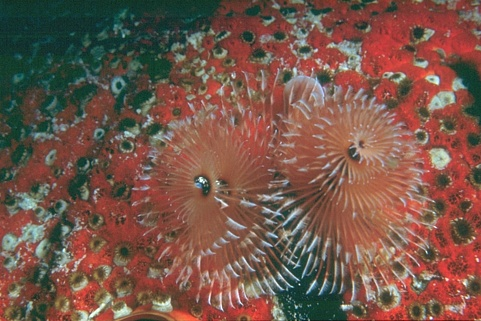
\includegraphics[width=73mm]{fig/Imagen3.jpg}}
%		\subfigure[Imagen Mejorada]{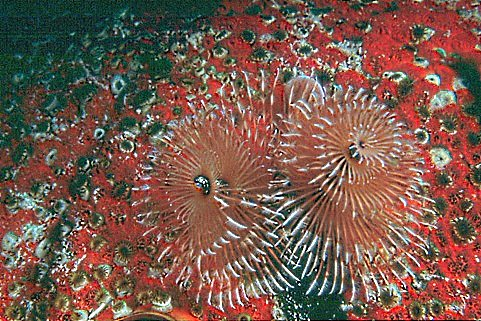
\includegraphics[width=73mm]{fig/Resultado3_3_4.jpg}}
%		  \caption{(a) Imagen con mejora de contraste aplicando 4 veces la ecuación \ref{contraste} con el método de ordenamiento propuesto}
%  \label{fig:mejora}
%\end{figure}

\begin{figure}
	\makebox[\linewidth][c]{%
		\begin{subfigure}[b]{0.5\textwidth}
			\centering
			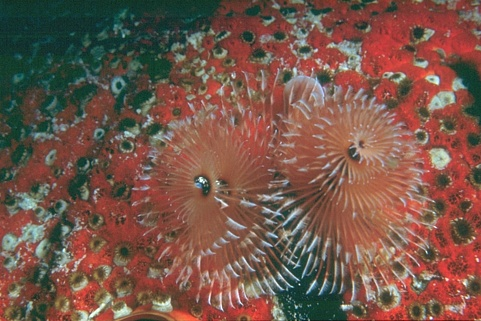
\includegraphics[width=0.8\textwidth]{fig/Imagen3.jpg}
			\caption{Imagen original}
			\label{fig:imagen_original_3}
		\end{subfigure}
	}\\
	\makebox[\linewidth][c]{%
		\begin{subfigure}[b]{0.5\textwidth}
			\centering
			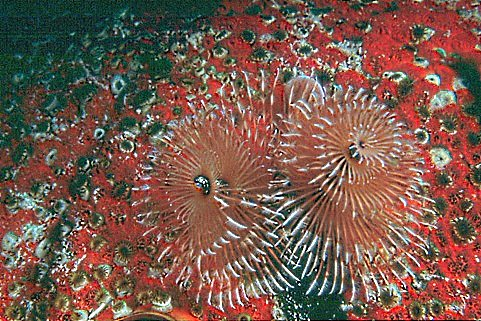
\includegraphics[width=0.8\textwidth]{fig/Resultado3_3_4.jpg}
			\caption{Imagen Mejorada}
			\label{fig:imagen_mejorada_3}
		\end{subfigure}
	}\\
	\caption{(a) Imagen con mejora de contraste aplicando 4 veces la ecuación \ref{contraste} con el método de ordenamiento propuesto}
  \label{fig:mejora}
\end{figure}


\subsection{Aplicación 3: Clasificación de texturas}
La granulometría y la covarianza morfológica son las principales herramientas morfológicas de caracterización de textura, ambas utilizan distribuciones de intensidad para describir las propiedades de las texturas \cite{lefevre2009beyond}.

%Los descriptores de textura morfológicos tienen la capacidad de describir efectivamente la regularidad y la direccionalidad por medio de la granulometría y la covarianza morfológica  \cite{hanbury2005illumination}. 

La manera en que la información de color y textura es incorporada al descriptor es estudiada en \cite{palm2004color,van2005parallel}. En este trabajo las herramientas morfológicas utilizan el enfoque integrativo donde la información de color y textura son procesadas conjuntamente.

La granulometría fue propuesta en \cite{matheron1975random} y es aplicado en la extracción de características y la estimación de tamaño \cite{vincent2000granulometries,soille2013morphological}. Consiste en una familia de aperturas $f \,\circ \, \lambda B $ de $n+1$ elementos incluyendo la imagen de entrada. Está parametrizada por el tamaño $\lambda$ creciente del elemento estructurante, donde $0 \leq \lambda \leq n $. Los valores son recolectados por una medida de evaluación que usualmente es el volumen $\mathrm{Vol}$:

\begin{equation}
G^{n}_{j}(f,\lambda)= \mathrm{Vol}([f\circ \lambda B ]_{j}) \; / \; \mathrm{Vol}(f_{j})
\end{equation}

Donde $j$ es el j-ésimo componente de la imagen a color $f$ y el volumen está definido como:
\begin{equation}
\mathrm{Vol}(f_j) = \sum_{\substack{u\in \{1, ..., M\}\\ v \in \{1, ..., N\}}}[f(u,v)]_{j} 
\end{equation}

La covarianza morfológica propuesta en \cite{matheron1975random,maragos1989pattern} denotada por $K$ de una imagen $f$, está definida como el volumen de la imagen $f$, luego de aplicarse la erosión $\varepsilon$ a partir de un par de pixeles $(u,v)$ y  $(u',v')$ separados por un vector $\vec{v}$ denotado por $P_{2,\vec{v}}$.\\
En la práctica $K $ es calculado aplicando la erosión $\varepsilon$ a la imagen original $f$ con el elemento estructurante $P_{2,\vec{v}}$ variando orientaciones y longitudes de $\vec{v}$, donde $n$ es el número de variaciones de $\vec{v}$. Su versión normalizada está dada por :
\begin{equation}
K^{n}_{j}(f,P_{2,\vec{v}})  = \mathrm{Vol}([\varepsilon(f,P_{2,\vec{v}})]_{j}) / \mathrm{Vol}(f_{j})
\end{equation}
Permite obtener una distribución de orientación y distancia de una imagen de textura \cite{aptoula2007morphological}.


%--------------------------------------------------------
\subsubsection{Resultados}
\label{sec:resultadosexperi}
Las pruebas fueron realizadas con la base de datos OutexTC13 compuesta por 1360 imágenes de dimensiones 128 $\times $ 128 píxeles, con 68 clases de texturas de superficies (Figura \ref{fig:outex13}) con 20 muestras de cada clase, donde el 50\% de cada clase es el conjunto de entrenamiento. Totalizan 680 imágenes de entrenamiento y prueba respectivamente \cite{ojala2002outex}.  
El clasificador utilizado fue el k-nn (k-nearest neighbors) utilizando distancia euclídea con k=1. 

\begin{figure}
	\centering
		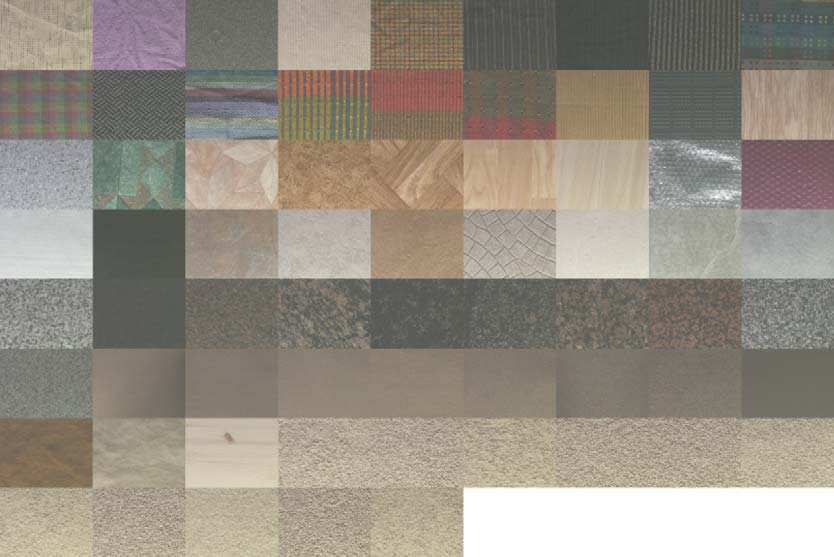
\includegraphics[scale=0.25]{fig/outex13.png}
	\caption{Muestras de textura OutexTC13}
	\label{fig:outex13}
\end{figure}

La finalidad del experimento fue obtener los porcentajes de clasificación utilizando los métodos de ordenación expuestos.
Se evaluaron varios parámetros estadísticos en la estrategia de orden propuesta en este trabajo.
%---configuracion de la granulometria
En las pruebas de granulometría se han utilizado elementos estructurantes de forma cuadrada de tamaño $\lambda$ y de lado $2\lambda+1$ píxeles, variando $\lambda$  de 1 a 15. Para cada elemento de la serie se calculan 15 valores para cada canal que posteriormente se concatenan. La elección del incremento simple de $\lambda$, está basado en que los incrementos menores proveen mejores resultados de clasificación \cite{de2006selecting}. 
Con respecto a la configuración de los parámetros de la propuesta, cada muestra de textura fue dividida en $2\times2$ sub-regiones y denotado por el sufijo W4. Esta división permite que cada muestra de textura sea dividida en partes iguales y perceptualmente similares. Se denota con el sufijo W0 cuando el dominio de la imagen es el propio elemento estructurante. 

%---configuracion de la covarianza morfologica
Para la covarianza morfológica las direcciones utilizadas fueron $0^{\circ}$, $45^{\circ}$, $90^{\circ}$, $135^{\circ}$ en combinación con distancias que varían de 1 a 20 píxeles.

Para cada elemento de la serie se calculan 80 valores para cada canal que luego se concatenan.
\begin{table}
\caption{ Resultados de clasificación por Métodos de Ordenamiento}
\label{tab:experiment1_t1}

\begin{tabular}{@{}lrr@{}}
\toprule
&\multicolumn{2}{c}{ \% Clasificados correctamente }\\
\cline{2-3}
\textbf{Ordenación } & \textbf{Covarianza} &\textbf{Granulometría } \\ 
\cmidrule{1-3}
%Marginal  & 85,78 & 88,68 \\ \hline
BM & 79,56 & 77,79 \\ \hline
ED & 81,91 & \textbf{84,11}  \\ \hline
LEX & 79,74 & 80,15 \\ \hline
ALEX & 76,32   &  69,12  \\ \hline
AMLEX &  81,62   &  81,30  \\ \hline
HLEX &  \textbf{83,97}  &  77,35  \\ \hline
DLAB  & \textbf{84,26}  & 72,35   \\ \hline
MEANW4 & 81,47 & 78,97 \\ \hline %$\mathrm{HST_{2}} $ Promedio 
%$\mathrm{HST_{2}} $ Entropía & 82,65 & \textbf{85,88} \\ \hline
SMOW4 & 82,50 & \textbf{85,44} \\ \hline %$\mathrm{HST_{2}} $
MO1W4 & 81,76 & 82,65 \\ \hline %$\mathrm{HST_{2}} $ Moda Min  
MO2W4 & 80,44 & 80,01 \\ \hline %$\mathrm{HST_{2}} $ Moda Max  
MAXW4 & 81,62 & 81,32 \\ \hline % $\mathrm{HST_{2}} $ Máximo
MINW4 & 81,47 & 83,38 \\ \hline %$\mathrm{HST_{2}} $ Mínimo 
VAR   & 81,76 &  83,97  \\ \hline 
MEANW0 & 81,91 & 78,82 \\ \hline %$\mathrm{HST}_{ b} $ Promedio
SMOW0 & \textbf{83,82} & \textbf{84,71} \\ \hline %$\mathrm{HST}_{b} $ Suavidad
MO1W0 & 82,01  & 83,23  \\ \hline %$\mathrm{HST_{2}} $ Moda Min  
MO2W0 & 81,21 &  81,36  \\ \hline %$\mathrm{HST_{2}} $ Moda Max  
MAXW0 & 81,32 & 81,06 \\ \hline %$\mathrm{HST}_{ b} $ 
MINW0 & 81,05 & 83,12 \\ \hline %$\mathrm{HST}_{ b} $
VARW0 & 83,09 &  82,21  \\ \hline 
%$\mathrm{HST_{2}} $ Desviación  & 82,01 & \textbf{85,02} \\ \hline
%$\mathrm{HST_{2}} $ Asimetria  & 81,91 & 83,09 \\ \hline
%$\mathrm{HST_{2}} $ Uniformidad & 80,74 & 80,44 \\ \hline
%$\mathrm{HST_{2}} $ Momento muestral & 79,56 & 60,88 \\ \hline
%$\mathrm{HST}_{ b} $ Desviación & \textbf{82,94} & \textbf{85,29} \\ \hline
%$\mathrm{HST}_{ b} $ Asimetría & \textbf{83,24} & \textbf{84,85} \\ \hline
%$\mathrm{HST_{2}} $ Energía & 82,35 & 79,56 \\ \hline
%$\mathrm{HST}_{ b} $ Entropía & 82,21 & 64,85 \\ \hline
%$\mathrm{HST}_{ b} $ Uniformidad & 80,59 & 80,29 \\ \hline
%$\mathrm{HST}_{ b} $ Momento Muestral & 46,47 & 62,78 \\ \hline
%$\mathrm{HST}_{ b} $ Energía & 82,03 & 81,47 \\ \hline
%$\mathrm{HST}_{ 2,4,8} $ Promedio & 81,62 & 84,12 \\ \hline
%$\mathrm{HST}_{ 2,4,8} $ Entropia & 82,79 & \textbf{85,74} \\ \hline
%$\mathrm{HST}_{ 2,4,8} $ Asimetría & 81,91 & 82,65 \\ \hline
%$\mathrm{HST}_{ 2,4,8} $ Desviación & 82,50 & 84,41 \\ \hline
%$\mathrm{HST}_{ 2,4,8} $ Uniformidad  & 80,74 & 80,59 \\ \hline
%$\mathrm{HST}_{ 2,4,8} $ Suavidad  & 82,50 & 84,56 \\ \hline
%$\mathrm{HST}_{ 2,4,8} $ Momento Muestral & 79,12 & 60,88 \\ \hline
%$\mathrm{HST}_{ 2,4,8} $ Moda  & 81,76 & 83,09 \\ \hline
%$\mathrm{HST}_{ 2,4,8} $ Máximo & 81,62 & 81,32 \\ \hline
%$\mathrm{HST}_{ 2,4,8} $ Mínimo & 81,47 & 83,53 \\ \hline
%$\mathrm{HST}_{ 2,4,8} $ Energía & 82,35 & 75,88 \\ \hline
\end{tabular}
\label{exper_ordenaciones}
\end{table}
%-  - - - - - - - - - - - - - -
En el Cuadro \ref{tab:experiment1_t1} los tres mejores resultados de cada método fueron marcados en negrita. La Covarianza Morfológica con los ordenamientos HLEX y DLAB tienen rendimientos superiores de $\approx 1\%$ con respecto a SMOW4 que presenta el mejor rendimiento en el espacio RGB. Los resultados son consistentes con los experimentos realizados en \cite{hanbury2005illumination} donde se obtienen mejores resultados en el espacio L*a*b en comparación al espacio RGB utilizando elementos estructurantes de longitud variante. Esto se debe a que en esos espacios de color la información cromática está separada de la luminosidad o intensidad. En experimentos mencionados en \cite{bianconi2011theoretical} sobre la percepción de la textura indican que la textura y el color se perciben de manera independiente. 
Con la granulometría el espacio RGB presenta mejores resultados con los ordenamientos SMOW4 y SMOW0, ambos superiores al ordenamiento ED en ($\approx 1,33 \% $). Por otra parte el ordenamiento ED provee resultados muy superiores a los ordenamientos BM, LEX, ALEX y AMLEX.

Los ordenamientos SMOW4 y SMOW0 (85,44\%, 84,71\%) exhiben los mejores resultados de clasificación (con granulometría) con respecto a los métodos de ordenamiento del estado del arte implementados. La división en $2\times2$ sub-regiones (W4) conducen a mejores resultados que usando W0.  

\section{Conclusiones y Trabajo Futuro}

En este trabajo se presenta una nueva estrategia de ordenamiento de colores RGB que es dependiente de la imagen. El ordenamiento se realiza por medio de extraer información del histograma de cada componente de color en cierto dominio de la imagen, y de esta manera poder asignar un peso a cada uno de ellos por medio de una transformación. Se presentaron dos estrategias simples de descomposición de dominios para extraer dicha información, una es extrayendo información de la misma ventana del filtro, y otra consiste en dividir la imagen en sub-regiones de mismo tamaño, tomando la intersección de ellos para cuando la ventana del filtro toma más de una sub-región.
Se realizaron pruebas para 3 aplicaciones de procesamiento de imágenes: Eliminación de ruido, estiramiento de contraste y caracterización texturas para su posterior clasificación.  Para estas dos últimas aplicaciones se utiliza matemática morfológica. Los operadores morfologicos en este caso son pseudo-operadores, ya que se no puede garantizar ciertas propiedades teóricas, como la idempotencia. 
Para la eliminación de ruido se utilizó el filtro mediana, consiguiendo mejores resultados con algunos pesos extraidos a diferentes métodos del estado del arte, tanto para ruido gaussiano, como speckle. Para el ruido sal y pimienta la distancia euclidiana al origen en el espacio de color RGB en la métrica MAE y la distancia euclidiana al origen en el espacio de color L*a*b* en la métrica CDS dieron mejores resultados al método propuesto con las diferentes informaciones extraidas de cada componente. 
Para la aplicación de mejora de contraste el método propuesto se mostró más eficiente según la métrica CEF a los diferentes métodos del estado del arte. En la última aplicación para caracterización de texturas utilizando la Covarianza Morfológica con los ordenamientos lexicográfico en el espacio de color HSI, comparando primero la I, luego la S, y por último la H (propuesto en \cite{ortiz2004gaussian}), la distancia euclidiana al color $(0,0,0)$ en el espacio de color L*a*b* \cite{ortiz2002procesamiento}  tienen rendimientos superiores a la propuesta. El método propuesto utilizando la suavidad como peso para cada componente  consigue mejores resultados  utilizando la granulometría como caracterización de texturas.
Como trabajo futuro se propone hacer un análisis exhaustivo de la importancia de descomposición de dominios para extraer información de cada componente de color. Se podrían hacer más experimentos en diferentes aplicaciones como segmentación o fusión de imágenes a color. Se podrían extraer otro tipo de información por cada componente como la Entropía o la Energía.
 


%Por lo tanto en $K^{TH}$, el contraste  entre las \'areas brillantes y oscuras de la imagen $f$ es mayor.

%En la actualidad existen varios operadores de contraste compuestos y multiescala a partir de la transformada top-hat \cite{bai2012toggle}. Como el objetivo de este trabajo no es crear un nuevo operador de contraste sino validar la estrategia de ordenamiento de color  usaremos la ecuaci\'on \ref{contraste} en la aplicaci\'on de mejoramiento de contraste. Con la misma se podr\'a comparar los diferentes trabajos del estado de arte y la propuesta en la secci\'on de experimentos.

%\section{Section title}
%\label{sec:1}
%Citation of \cite{trouiller2002drug}.
%\subsection{Subsection title}
%\label{sec:2}
%as required. Don't forget to give each section
%and subsection a unique label (see Sect.~\ref{sec:1}).
%\paragraph{Paragraph headings} Use paragraph headings as needed.
%\begin{equation}
%a^2+b^2=c^2
%\end{equation}

% For one-column wide figures use
%\begin{figure}
%\centering
% Use the relevant command to insert your figure file.
% For example, with the graphicx package use
%  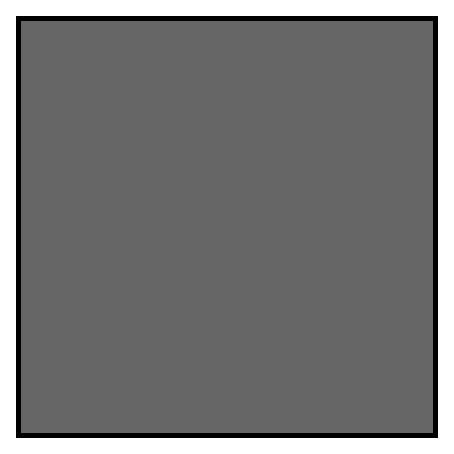
\includegraphics{example.eps}
% figure caption is below the figure
%\caption{Please write your figure caption here}
%\label{fig:1}       % Give a unique label
%\end{figure}
%
% For two-column wide figures use
%\begin{figure}
%\centering
% Use the relevant command to insert your figure file.
% For example, with the graphicx package use
%  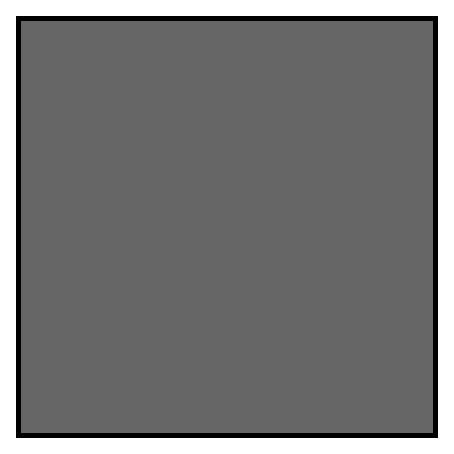
\includegraphics[width=0.75\textwidth]{example.eps}
% figure caption is below the figure
%\caption{Please write your figure caption here}
%\label{fig:2}       % Give a unique label
%\end{figure}
%
% For tables use
%\begin{table}[h]
% table caption is above the table
%\caption{Please write your table caption here}
%\centering
%\label{tab:1}       % Give a unique label
% For LaTeX tables use
%\begin{tabular}{lll}
%\hline\noalign{\smallskip}
%first & second & third  \\
%\noalign{\smallskip}\hline\noalign{\smallskip}
%number & number & number \\
%number & number & number \\
%\noalign{\smallskip}\hline
%\end{tabular}
%\end{table}


%\begin{acknowledgements}
%If you'd like to thank anyone, place your comments here
%and remove the percent signs.
%\end{acknowledgements}

% BibTeX users please use
\bibliographystyle{spbasic}
\bibliography{sample}   % name your BibTeX data base

% Non-BibTeX users please use
%\begin{thebibliography}{}
%
% and use \bibitem to create references. Consult the Instructions
% for authors for reference list style.
%
% Format for Journal Reference
%\bibitem[Author I(1999)]{RefJ}
%Author I (year) Article title. Journal Title-Abbreviated Vol: pp--pp
% Format for books
%\bibitem[Author and Smith(2001)]{RefB}
%Author I, Smith J (year) Book title. Publisher, Place, pp numbers
% etc
%\end{thebibliography}

\end{document}
% end of file template.tex
